\documentclass[conference]{IEEEtran}

\usepackage{fancyhdr}
\usepackage{graphicx}
\usepackage{algorithm}
\usepackage{algorithmic}
\usepackage{booktabs}
\usepackage{amsmath}
\usepackage[flushleft]{threeparttable}
\usepackage{multirow}
\usepackage{cases}
\usepackage{listings}
\lstset{language=C++,
    basicstyle=\ttfamily \footnotesize,
    keywordstyle=\color{black}\ttfamily,
    stringstyle=\color{black}\ttfamily,
    commentstyle=\color{gray}\ttfamily,
    morecomment=[s][\color{blue}]{/**}{**/},
    showstringspaces=false,
    showtabs=false,
    captionpos=b,
    numbers=left
}

\hyphenation{cluster computational-biology short-read-mapping}


\begin{document}

\title{S-Aligner: Ultrascalable read mapping on Sunway Taihu Light}

\author{\IEEEauthorblockN{Xiaohui Duan, Kai Xu, Yuandong Chan}
\IEEEauthorblockA{
Shandong University\\
Jinan, China\\
Email: \{sunrise.duan, xu\_kai, yuandong.c\}@mail.sdu.edu.cn}
\and
\IEEEauthorblockN{Christian Hundt, Bertil Schmidt}
\IEEEauthorblockA{Johannes Gutenberg University\\
Mainz, Germany\\
Email: \{hundt, bertil.schmidt\}@uni-mainz.de}
\and
\IEEEauthorblockN{Pavan Balaji}
\IEEEauthorblockA{Argonne National Laboratory\\
Lemont, Illinois, USA\\
Email: balaji@anl.gov}
\and
\IEEEauthorblockN{Weiguo Liu}
\IEEEauthorblockA{Shandong University\\
Jinan, China\\
Email: weiguo.liu@sdu.edu.cn\\
}
}

\maketitle


\begin{abstract}

  The availability and amount of sequenced genomes have been rapidly
  growing in recent years because of the adoption of next-generation
  sequencing (NGS) technologies that enable high-throughput
  short-read generation at highly competitive cost. Since this trend
  is expected to continue in the foreseeable future, the design and
  implementation of efficient and scalable NGS bioinformatics
  algorithms are important to research and industrial applications.
  In this paper, we introduce S-Aligner---a highly scalable read
  mapper designed for the \emph{Sunway Taihu Light} supercomputer and
  its fourth-generation ShenWei many-core architecture
  (SW26010). S-Aligner employs a combination of optimization
  techniques to overcome both the memory-bound and the compute-bound
  bottlenecks in the read mapping algorithm. In order to make full use
  of the compute power of Sunway Taihu Light, our design employs three
  levels of parallelism: (1) internode parallelism using MPI based on
  a task-grid pattern, (2) intranode parallelism using
  multithreading and asynchronous data transfer to fully utilize all
  260 cores of the SW26010 many-core processor, and (3) vectorization
  to exploit the available 256-bit SIMD vector registers.  Moreover,
  we have employed asynchronous access patterns and data-sharing
  strategies during file I/O to overcome bandwidth limitations of the
  network file system. Our performance evaluation demonstrates that
  S-Aligner scales almost linearly with approximately 95\% efficiency
  for up to 13,312 nodes (concurrently harnessing more than 3 million
  compute cores). Furthermore, our implementation on a single node
  outperforms the established RazerS3 mapper running on a platform
  with eight Intel Xeon E7-8860v3 CPUs while achieving highly
  competitive alignment accuracy.

\end{abstract}

\IEEEpeerreviewmaketitle

\section{Introduction}
\label{Introduction}

{\em Next-generation sequencing} (NGS) technologies have
revolutionized the field of computational biology because of their
massive throughput at highly competitive cost. Today, NGS data is
processed in almost every field of bioinformatics, with important
applications including personalized cancer treatment and precision
medicine.  Modern NGS instruments such as Illumina sequencers
\cite{reviewngs} enable the recording of billions of short DNA
fragments per day. The produced \emph{short reads} are usually only a
few hundred base pairs (bps) in length compared with complete genomes
of typical mammals covering billions of nucleotides. In order to
further analyze the set of delocalized reads, they are typically
mapped to a given reference genome by computing base-pair-level
alignments to determine their original positions. This exhaustive
probing of possible alignments is a compute-heavy task and thus
justifies the need for massively parallel and efficient computation
patterns. Moreover, read alignment (or mapping) is crucial for many
DNA sequence analysis pipelines such as genotyping, the discovery of
single nucleotide polymorphism, or personal genomics.

The na\"ive computation of optimal local alignments between each read
and the reference genome is considered prohibitive because of the
demanding time complexity of the Smith-Waterman algorithm \cite{sw}
that is proportional to the product of the sequences' lengths. Thus,
methods based on a {\em seed-and-extend} approach are typically
employed to dramatically reduce the number of alignment positions by
considering only those regions in the reference genome that contain
an exact occurrence of a substring of a read. Among existing read
mappers are two predominant operation modes: {\em any-best}
and {\em all}. Bowtie2 \cite{bowtie2}, BWA \cite{bwa}, GEM \cite{gem},
and CUSHAW \cite{cushaw} run in {\em any-best} mode, which determines
only one or a few best alignments (also called {\em intervals}) of
each read to the reference genome. Other mappers such as RazerS3
\cite{razers3}, Hobbes2 \cite{hobbes2}, BitMapper \cite{bitmapper},
and mrFAST \cite{mrfast} operate in {\em all} mode, which reports all
intervals satisfying a certain constraint, for example, compliance
with a predefined edit distance threshold.  Because of their extensive
nature, all-mappers demand far more computational resources than their
any-best counterparts do. Nevertheless, when studying gene innovation or
phenotypic variation, the complete list of alignments is crucial for a
thorough analysis.

Consequently, we pursue the design of an all-mapper in order to
support a wide range of biomedical applications. Associated runtimes
can be dramatically reduced if we target clusters with a large number
of compute nodes. In the recent past, the prevalent trend in
supercomputing has favored heterogeneous nodes featuring attached
coprocessors, such as GPUs or Xeon Phi architectures, because of their
vast compute capabilities and low energy footprint. A similar
architecture has recently been introduced with the \emph{Sunway Taihu
  Light} supercomputer, which is based on the neo-heterogeneous
SW26010 many-core processor. This cluster consists of 40,960
nodes. Each node provides 260 compute cores organized in four {\em
  compute groups} (CGs). A total of 10,649,600 cores provides Linpack
performance of up to 93 PFlop/s, rendering it the world's fastest
supercomputer in the Top500 list of November 2016.

In this paper, we introduce S-Aligner---a highly scalable read mapper
targeting the Sunway Taihu Light supercomputer and its SW26010
architecture. To the best of our knowledge, we are the first to
investigate the applicability and scalability of read mapping on this
architecture. Our approach relies on four major contributions. First,
we provide an efficient implementation of Myers' bit-parallel string
matching algorithm that harnesses the full parallelization and
vectorization potential of the SW26010 many-core processor. Our new
implementation is three orders of magnitude faster than a na\"ive
single-threaded Myers version. Second, we exploit fast local device
memory via direct memory access (DMA) intrinsics for intra-CG communication, which results in
a 22$\times$ speedup compared with the non-DMA variant. Third, we propose a
highly scalable inter-CG communication scheme. This
results in a parallelization efficiency of over 95\% when using 53,248
CGs. Fourth, we employ asynchronous file loading and data-sharing
strategies to effectively hide the latency of the network file
system. We expect that the presented techniques can guide the
design and implementation of similar types of applications on the
neo-heterogeneous many-core cluster architecture of Sunway Taihu
Light.

The rest of this paper is organized as follows: Section~\ref{Related
  Work} describes required background about the Sunway Taihu Light
architecture, related work, and the seed-and-extend approach to read
mapping. Details of the design and implementation of S-Aligner are
presented in Section~\ref{Implementation}. Performance evaluations in
terms of speed, scalability, and alignment quality are carried out in
Section~\ref{Evaluation}. Section~\ref{Conclusion} summarizes our
conclusions.

\section{Background}
\label{Related Work}

\subsection{Sunway Taihu Light Architecture}
\label{Sunway Taihu Light}

The Sunway Taihu Light has been manufactured by the National Research
Center of Parallel Computer Engineering \& Technology (NRCPC) of the
People's Republic of China and is located at the Wuxi Supercomputing
Center. It provides a theoretical peak performance of 125 PFlop/s and
an effective performance-to-power ratio of over 6 GFlop/s per watt. It
consists of 40,960 nodes with 1.4 PB attached memory. The
interconnection network provides roughly 70 TB/s bisection bandwidth
and 12 GB/s point-to-point communication bandwidth.

\begin{figure}[!htb]
  \begin{center}
    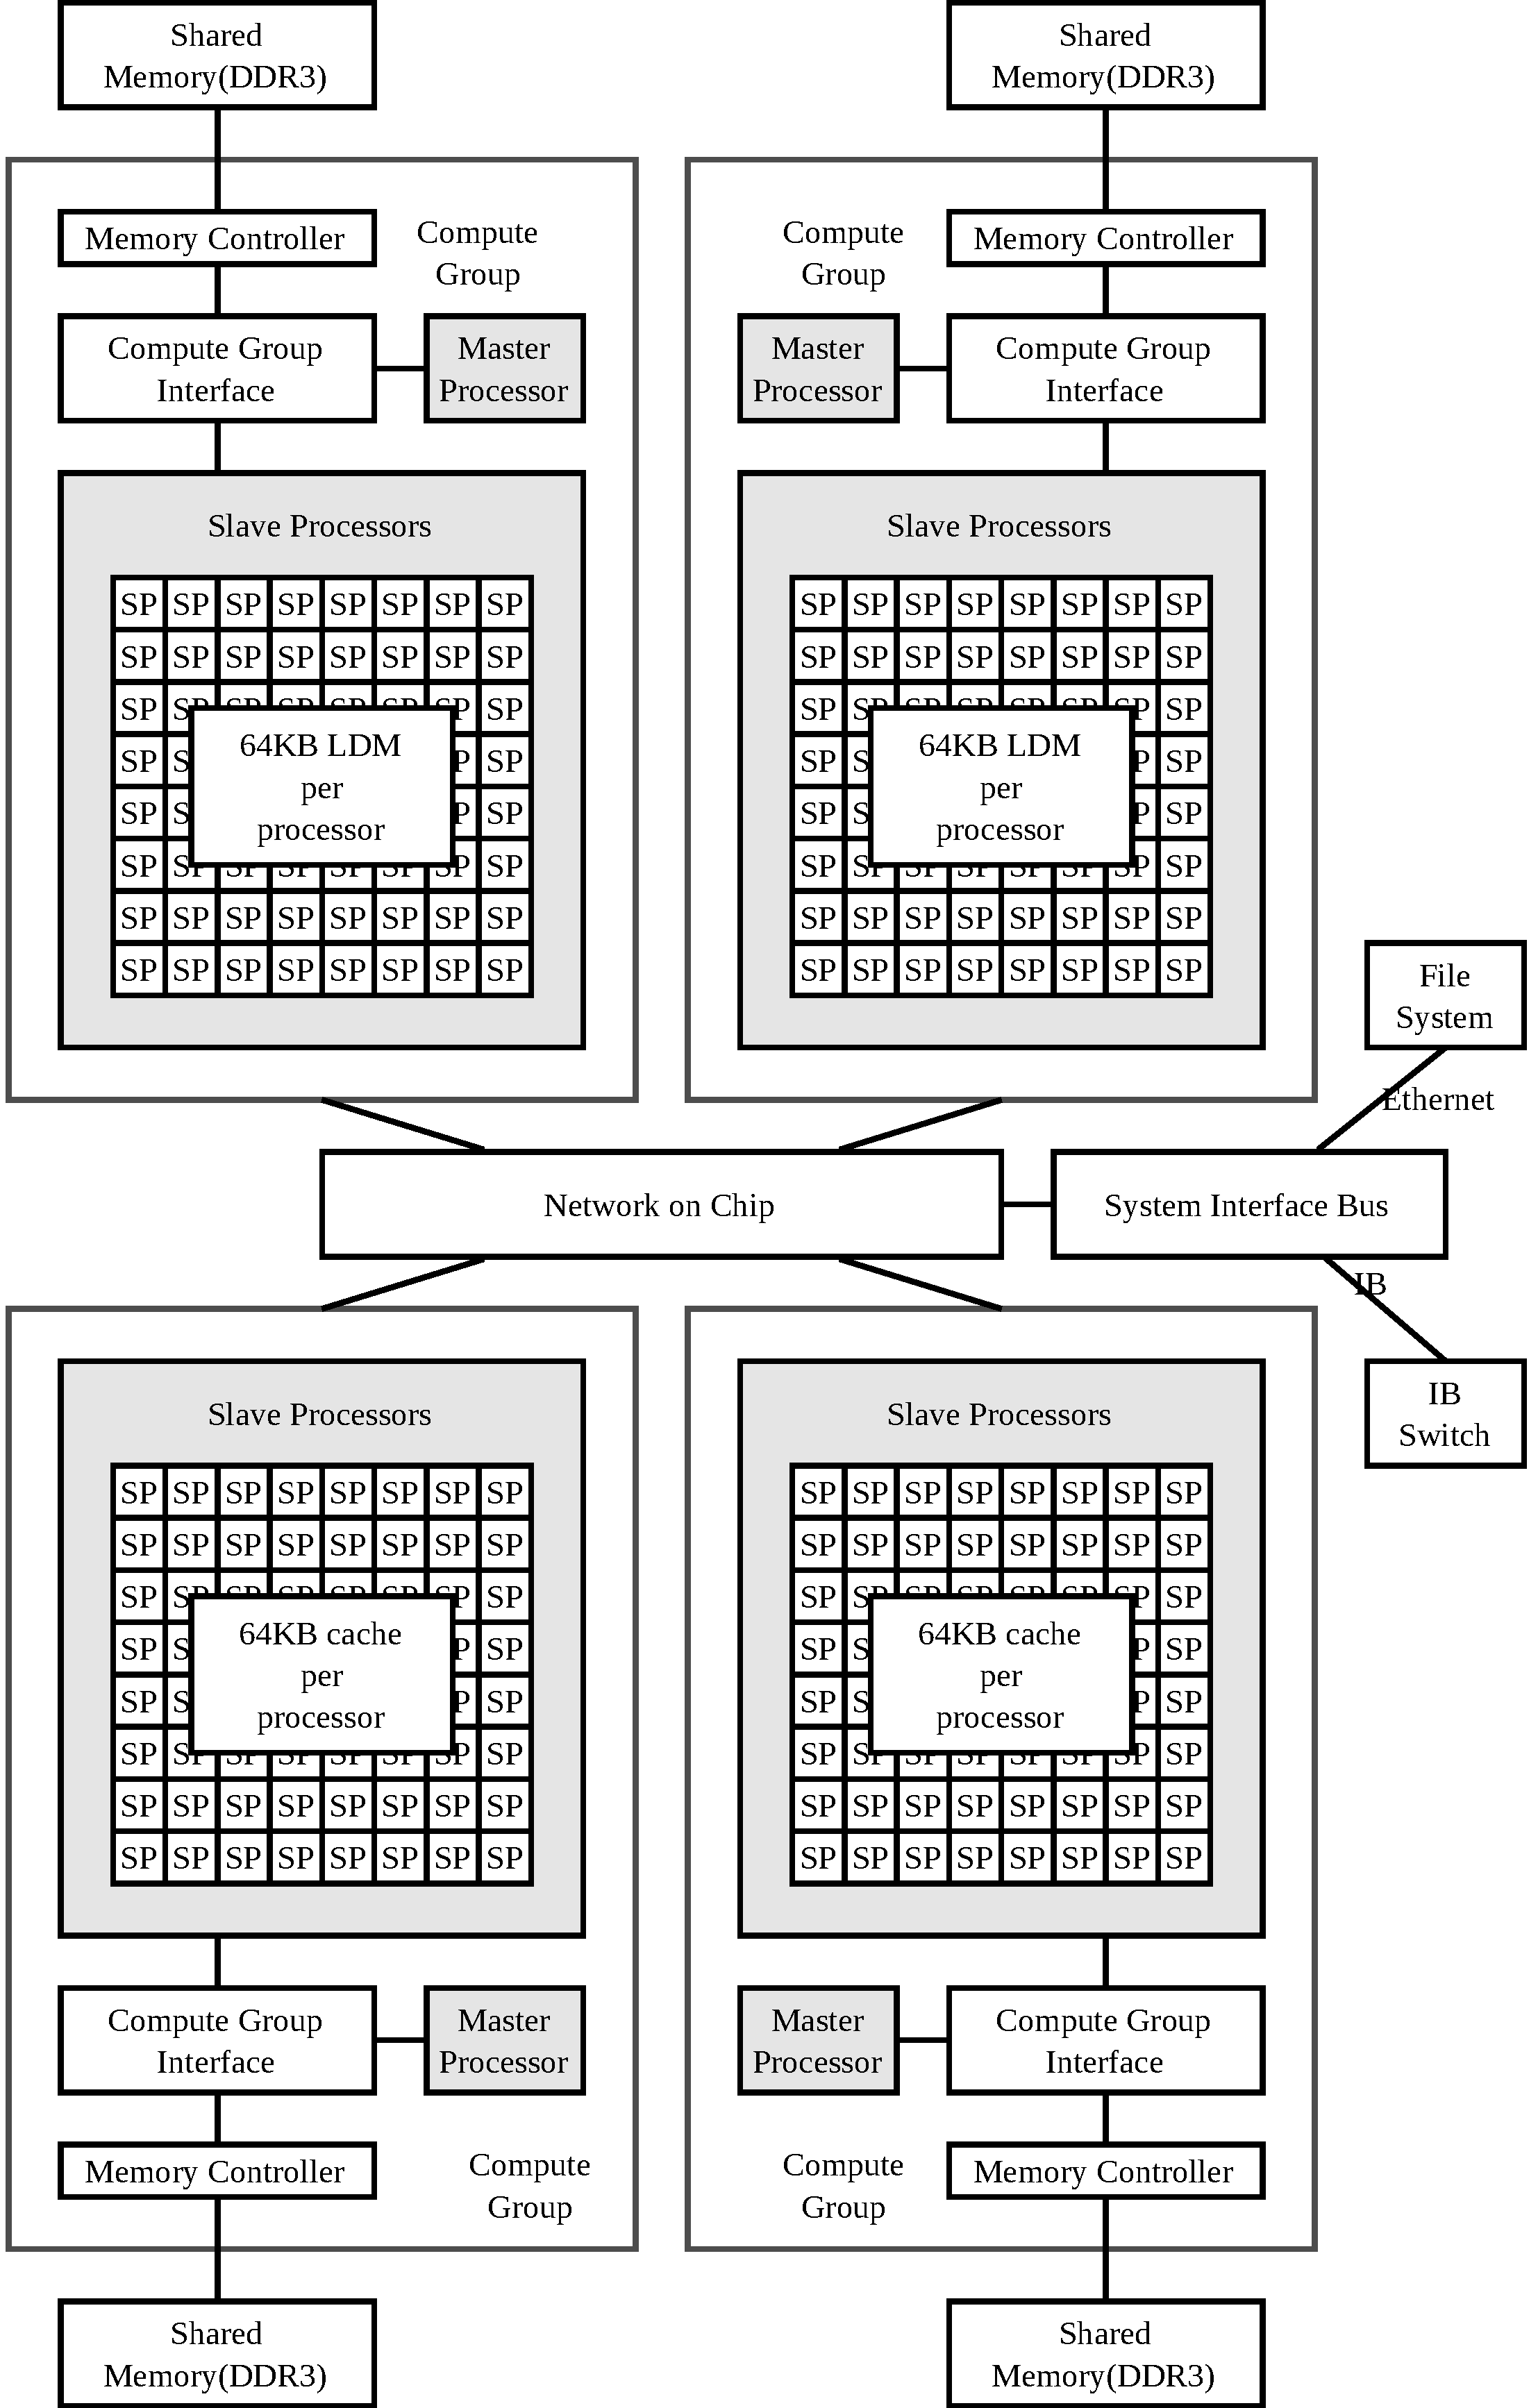
\includegraphics[width=\linewidth]{figures/SW26010}
    \caption{Architecture of the SW26010 processor, which is
      partitioned into four CGs.}
    \label{fig:SW26010}
  \end{center}
\end{figure}

Each node is equipped with a single SW26010 processor that is
subdivided into four {\em compute groups} (CGs). A CG is the basic
unit that can be addressed by the job scheduling system. Each CG
consists of a single {\em master processor} (MP), 64 {\em slave
  processors} (SPs), and 8 GB of attached DDR3 shared memory. All
nodes can access a shared network file system for loading and storing
data. The operating system is a customized Linux flavor running on the
MP.  Users may manually launch threads on the SPs in order to
parallelize compute-heavy portions of their code. Both the MP and 64
SPs support ShenWei's RISC basic instruction set, which provides
scalar and SIMD operations. Moreover, reduction primitives can be
called exclusively on the MP, while the SPs exhibit specialized
intrinsics for high-precision integer arithmetic. The 8 GB attached
shared memory can be accessed by both the MP and the 64 SPs via a
memory controller with a shared bandwidth of approximately 136
GB/s. The MP has its own cache (L1 and L2), and each SP can access 64
KB of fast {\em local device memory} (LDM). Data residing in shared
memory can be written to LDM using DMA intrinsics and subsequently
communicated via a broadcast to the LDM of other
SPs. Figure~\ref{fig:SW26010} shows the described hardware layout.

ShenWei's SIMD instruction set features 256-bit wide vector types and
a set of corresponding intrinsics provided by the \emph{ShenWei 5
  Compiler Collection}.  The MPI library (Sunway MPI) is a derivative
of the MPICH implementation, and is compliant with the MPI-3 standard.
Basic threading capabilities for the SPs are provided by the
\emph{athread} library.

\subsection{Related Work}

We are not the first to parallelize read mapping on a compute
cluster. Among the earliest tools are pBWA \cite{pbwa} and pMap
\cite{pmap}. pBWA is an MPI implementation of Version 0.5.9 of the BWA
aligner while pMap provides an MPI-based framework for the concurrent
execution of popular aligners such as BWA \cite{bwa} and Bowtie
\cite{bowtie}. Other implementations exploit MapReduce frameworks, for
example, the Hadoop-based SEAL \cite{seal} and BigBWA \cite{bigbwa}
tools or the Spark-based SparkBWA suite \cite{sparkBWA}, in order to
guarantee fault tolerance. Unfortunately, all these approaches suffer
from insufficient scalability when executed on hundreds of nodes. The
metaframework parSRA \cite{parSRA} is designed for read mappers
written in UPC++.  It combines dynamic scheduling and a virtual file
system layer for read distribution to overcome the limitations imposed
by pMap and MapReduce-based approaches. merAligner \cite{merAligner}
and CUSHAW3-UPC++ \cite{cushaw3upc} are other PGAS-based short-read
aligners written in UPC; both demonstrate good scalability. Although
pMap and parSRA allow for the execution of single node GPU aligners
such as nvBowtie \cite{nvBio}, none of the cited tools is explicitly
designed for heterogeneous clusters consisting of thousands of
many-core processors. Furthermore, all previous approaches target
traditional hardware architectures.

To the best of our knowledge, S-Aligner is the first attempt to
implement a fully scalable read mapper specifically designed to fit
the characteristics of Sunway Taihu Light. Previous algorithms mapped
onto this novel supercomputer have focused mainly on application
domains outside bioinformatics, such as Earth system modeling, ocean
surface wave modeling, atomistic simulation, and phase-field
simulation \cite{sunway}.

\subsection{Seed-and-Extend Approach}

Consider a set of reads ${\cal R}$, a reference genome $G$, and an
error threshold $e$. The read mapping problem can be defined as
follows: Find all substrings $g$ of $G$ that are within edit distance
$e$ to some read $R \in {\cal R}$. We call such occurrences $g$ in $G$
{\em matches}.

This problem can be solved by a classical {\em dynamic programming}
(DP) approach that calculates the semi-global alignment between each
$R \in {\cal R}$ and $G$. Unfortunately, each alignment results in a
time complexity proportional to the product of the sequences' lengths,
which renders intractable the alignment of a large number of short
reads to a reference genome a few billion letters long.  In order to
address this problem, most state-of-the art solutions \cite{Reinert}
employ the {\em seed-and-extend} approach, which follows a three-stage
pipeline.

\begin{description}

\item[Stage 1: Filtration.] This stage identifies promising candidate
  regions (called {\em seeds}) for each read in $G$. A popular
  strategy in order to discard large regions of $G$ is based on the
  fact that if a read $R \in {\cal R}$ is divided into $e+1$
  non-overlapping $q$-grams (substrings of length $q = \lfloor \lvert
  R\rvert\ /(e+1) \rfloor$), then (according to the pigeonhole
  principle) at least one of them occurs exactly in a match. Such
  occurrences can be identified quickly by looking them up in
  precomputed $q$-gram index data structure (also called the {\em
    reference genome index}), which stores all substrings of length
  $q$ of $G$.

\item[Stage 2. Verification.] This stage determines whether a seed can
  actually be extended to a full match within edit distance $e$. This
  requires the implementation of a {\em verification} algorithm in
  order to analyze the vicinity of each seed. Most mappers typically
  apply fast versions of DP-based algorithms for this step.

\item[Stage 3. Alignment.] This stage generates the base-pair level
  alignment information of a read and its verified intervals in $G$.

\end{description}

Established all-mappers such as RazerS3 \cite{razers3} and mrFAST
\cite{mrfast} follow this pipeline. Our profiling of RazerS3 and
mrFAST using a typical benchmark data set including the human
reference HG19 and 1 million simulated Illumina reads (with a read
length of 100 bps) reveals that Stage 2 occupies 67\% and 93\% of the
overall runtime, respectively. This shows that a fast implementation
of Myers' bit-parallel algorithm for computing the edit distance
between a read and an interval is a crucial component when designing
efficient all-mappers.

Consider two strings $s$ and $s^\prime$ of length $n$ and $m$,
respectively. Their {\em edit distance} is the minimum number of point
mutations (i.e. insertions, deletions, or substitutions) required to
transform $s$ into $s^\prime$. It can be determined by relaxing the
cells of a cost matrix $C$ of size $(n+1) \times (m+1)$ according to
the recurrence relation shown in Equation~\ref{update_scheme}, where
$0 < i \le n$ , $0 < j \le m$ and the {\em characteristic function}
$\chi (x \ne y)$ being 1 if $x \ne y$, and 0 otherwise. Initial
conditions are set to $C[i,0] = i$, $C[0,j] = j$, and $C[0,0] = 0$.

\begin{align}
  \label{update_scheme} 
  C[i,j]=\min \begin{cases} C[i-1,j-1]+\chi(s_{i-1} \neq s'_{j-1})\\
    C[i-1,j]+1 \\
    C[i,j-1]+1
  \end{cases}
\end{align}

Myers proposed a bit-vector algorithm \cite{myers} that exploits bit
parallelism by encoding the differences (deltas) between adjacent rows
and columns in the cost matrix $C$ as defined in
Equation~\ref{delta_update}, where $\varDelta h_{i,j}$, $\varDelta
v_{i,j}$, and $\varDelta d_{i,j}$ are the discrete derivatives of
$C[i, j]$ in the horizontal, vertical, and diagonal direction,
respectively.

\begin{align} \label{delta_update}
  \varDelta v_{i,j}&=C[i,j]-C[i-1,j]   &&\in \{0, \pm1\} \nonumber\\
  \varDelta h_{i,j}&=C[i,j]-C[i,j-1]   &&\in \{0, \pm1\} \\
  \varDelta d_{i,j}&=C[i,j]-C[i-1,j-1] &&\in \{0, +1\}   \nonumber
\end{align}

Note that the absolute values in Equation~\ref{delta_update} are
either 0 or 1. Thus, we can encode the relatively small state space
with the help of five vectors using one-hot
encoding. Figure~\ref{BitDP} shows an example for the encoding of the
vertical derivative $\varDelta v$ and its associated one-hot
representations $V^+$ and $V^-$.  With this bit-vector representation
the cell updates can be rewritten in terms of logical operations as
shown in Equation~\ref{one-hot-myers}:

\begin{alignat}{100}
  \label{one-hot-myers}
  H^-_{i, j} &= \chi(\varDelta h_{i, j} &&= -1)            &&= V^+_{i, j-1} &&\land D^0_{i, j} \nonumber\\
  V^-_{i, j} &= \chi(\varDelta v_{i, j} &&= -1)            &&= H^+_{i-1, j} &&\land D^0_{i, j} \nonumber\\
  H^+_{i, j} &= \chi(\varDelta h_{i, j} &&= +1)            &&= V^-_{i, j-1} &&\lor \lnot(V^+_{i, j-1} \,\lor D^0_{i, j}) \\
  V^+_{i, j} &= \chi(\varDelta v_{i, j} &&= +1)            &&= H^-_{i-1, j} &&\lor \lnot(H^+_{i-1, j}   \lor D^0_{i, j}) \nonumber\\
  D^0_{i,j}  &= \chi(\varDelta d_{i, j} &&= \phantom{+}0)  &&= V^-_{i, j-1} &&\lor H^-_{i-1, j} \lor \chi(s_{i-1} = s'_{j-1}) \nonumber 
\end{alignat}

\begin{figure}[!htb]
  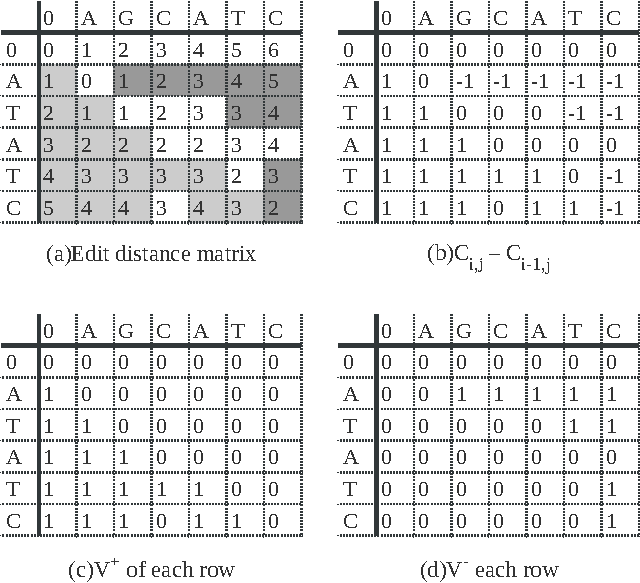
\includegraphics[width=1\linewidth]{figures/BitDP}
  \caption{Relations between the original matrix, $\varDelta v$,
    $V^+$, and $V^-$.  Here (a) shows the original score matrix;
    light-shaded cells indicate $\varDelta v_{i,j}=+1$ while heavily
    shaded cells correspond to $\varDelta v_{i,j}=-1$. The vertical
    derivative $\varDelta v$ shown in (b) is subsequently one-hot
    encoded by the bit vectors $V^+$ and $V^-$ in (c) and (d),
    respectively.}
  \label{BitDP}
\end{figure}

\section{Design of S-Aligner}
\label{Implementation}

This section describes the implementation of both the inter-CG and
intra-CG parallelism for the S-Aligner. Also discussed is our
bit-level encoding strategy and the exploitation of local device
memory.

\subsection{Large-Scale Inter-CG Parallelization}

\begin{figure}[!htb]
  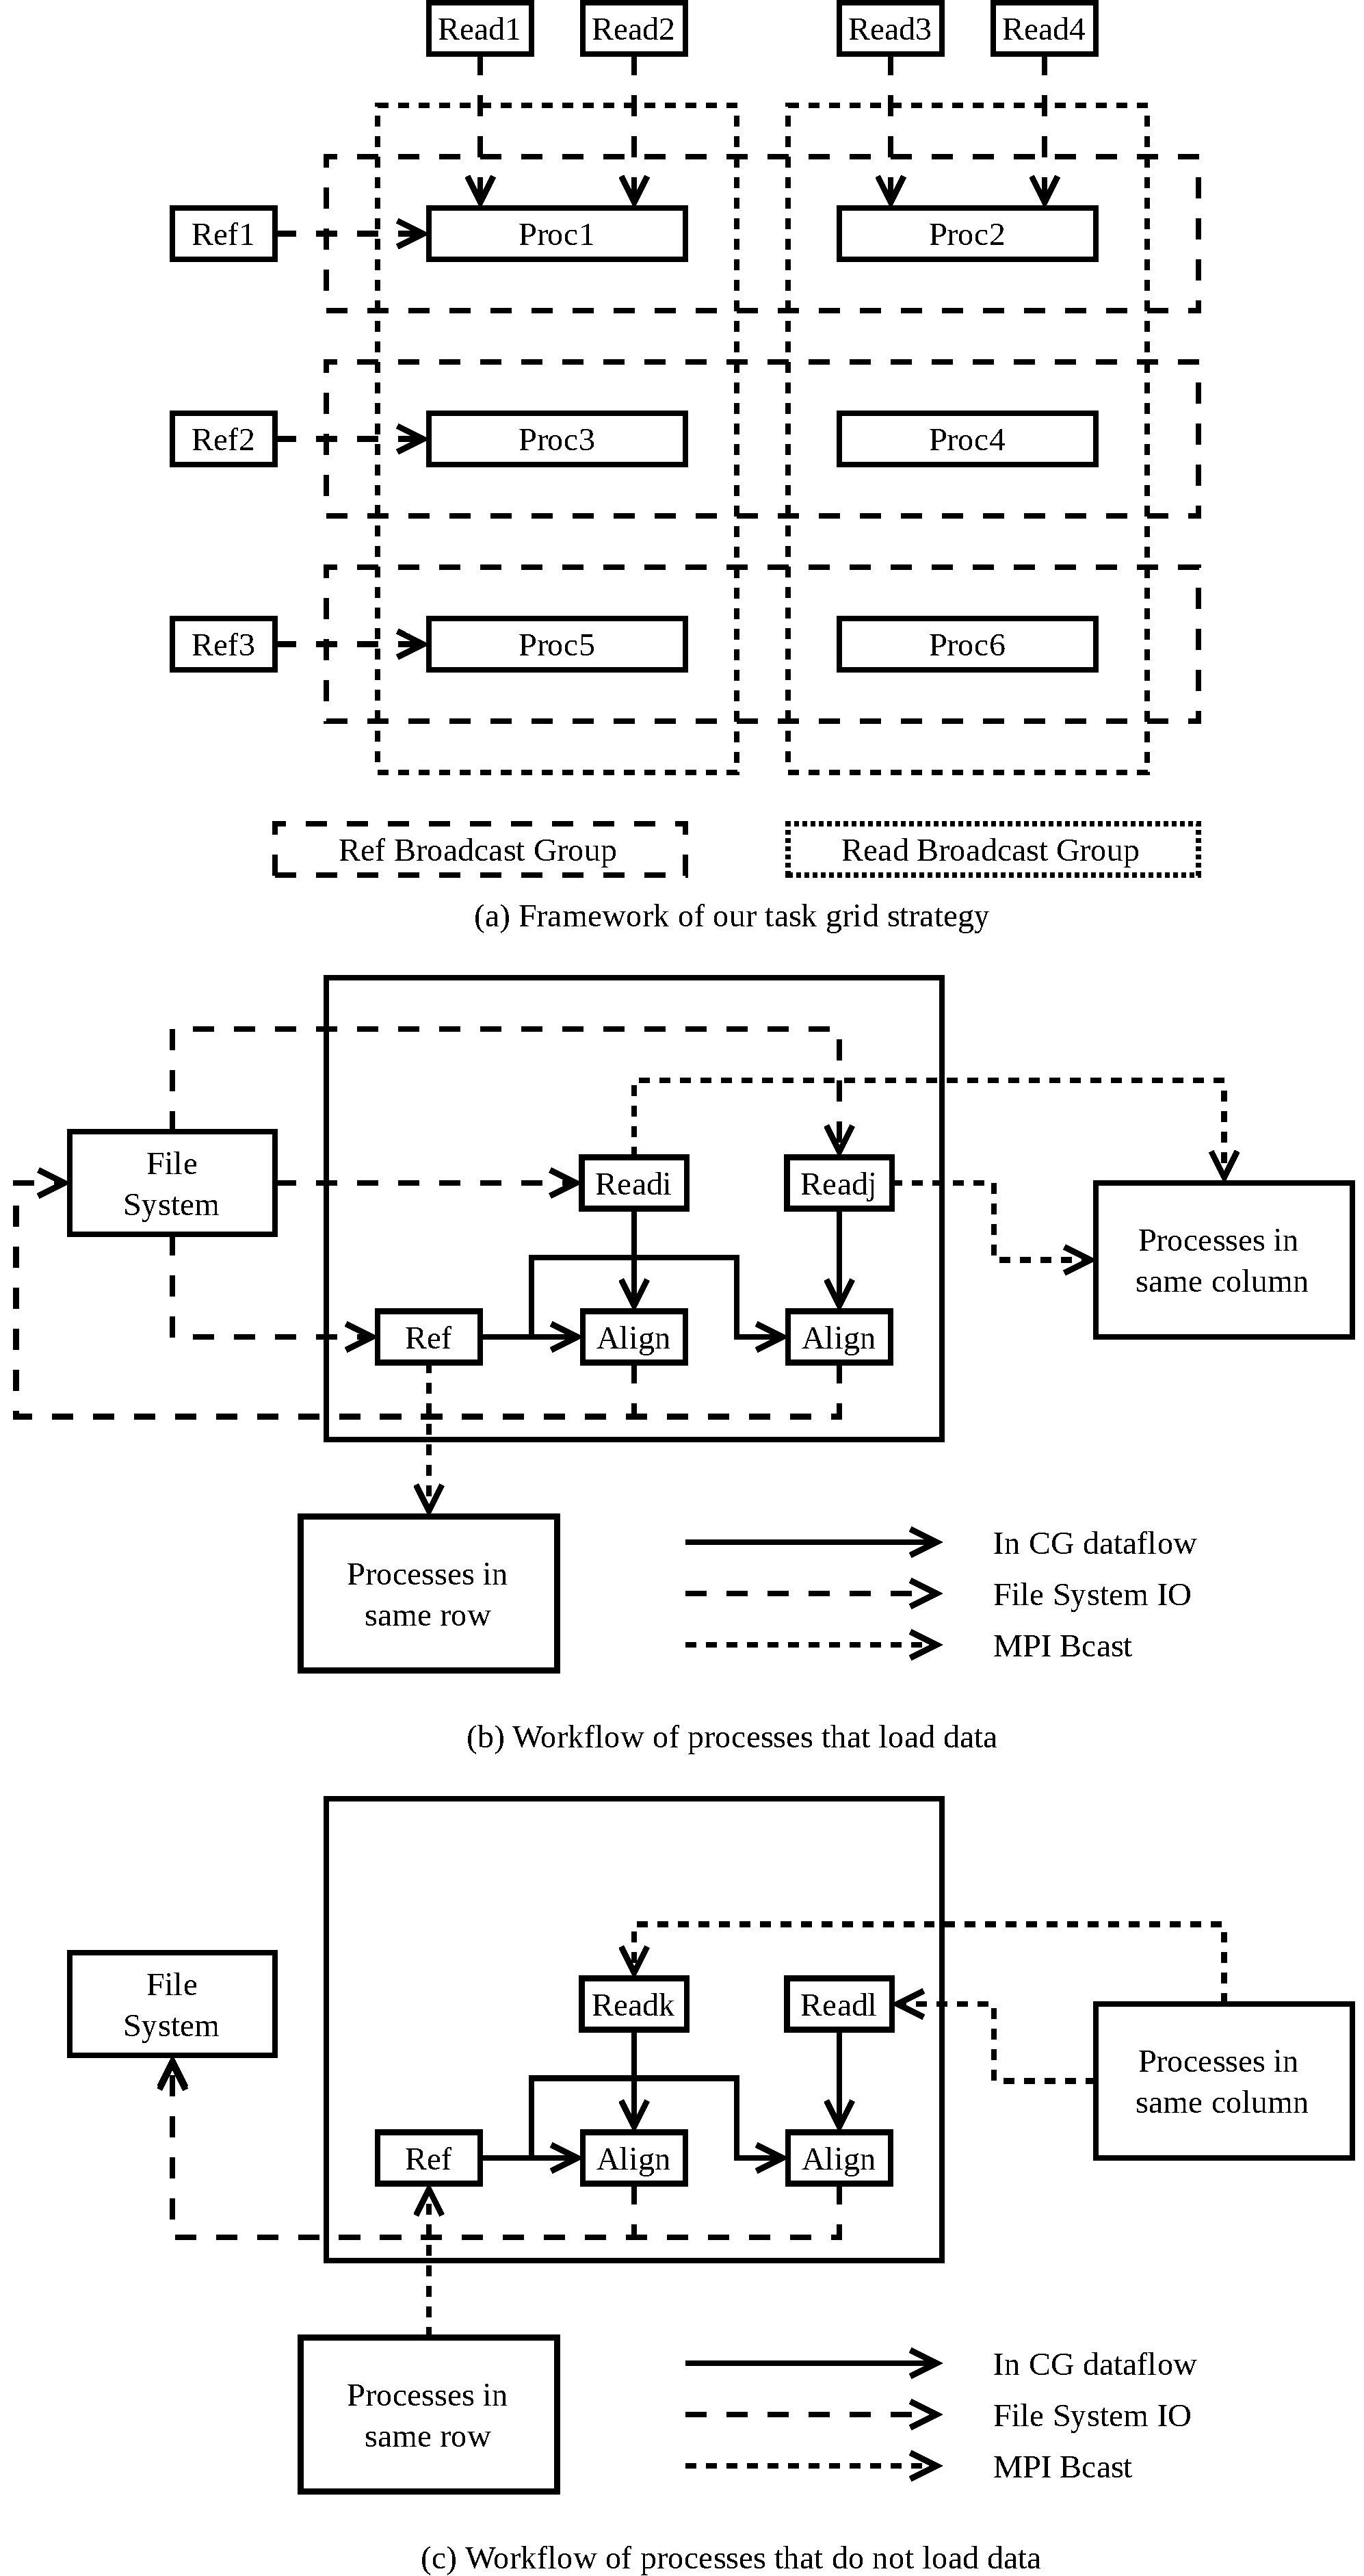
\includegraphics[width=\linewidth]{figures/GridNew}
  \caption{Our task-partitioning and file-loading strategy: (a)
    overall design; (b) and (c) detailed behavior of processes.}
  \label{TaskGrid}
\end{figure}

The highest level of parallelization employs a coarse-grained
partitioning scheme over a block distribution of reads and reference
genome using MPI. In our experiments we process up to 1.6 TB of read
data using up to 13,312 SW26010 nodes executing more than 50,000
dispatched processes. Thus, a na\"{\i}ve partitioning of the read file
into 50,000 pieces of approximately 32 MB size is not a suitable
solution because of the excessive data replication of the reference
genome index. Instead, we employ a partitioning strategy based on a
{\em task grid pattern} for the inter-CG parallelization by
concurrently assigning pairs of reference genome blocks and read
chunks to individual CGs. The two dimensions of the grid are spanned
by the reference block identifiers (rows) and read chunk identifiers
(columns) as shown in Figure \ref{TaskGrid}(a). Thus, processes in the
same row share a unique reference genome (index) block while processes
within a column use the same read chunk. Each process executes several
cells in one row in order to avoid replication of the relatively big
reference index.

\begin{figure}[!htb]
  \begin{center}
    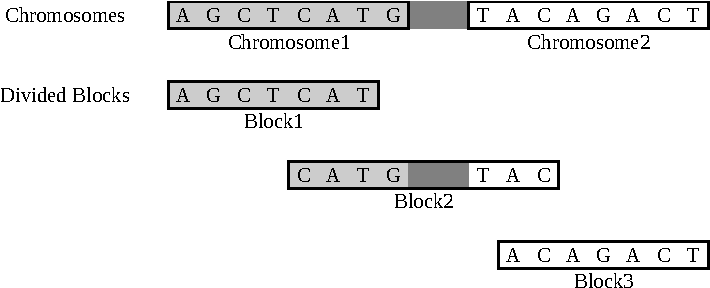
\includegraphics[width=0.9\linewidth]{figures/RefDiv}
    \caption{Exemplary partitioning of a reference genome based on
      concatenation and padded splits.}
    \label{RefDiv}
  \end{center}
\end{figure}

The read input file is partitioned into chunks of fixed size. This can
be easily achieved by splitting by lines. For the reference genome, we
first concatenate the individual chromosomes to form one long
string. We then divide it into blocks of suitable size according to
the memory capacity of a CG ($\approx$300 million bps per block). Note
that this partitioning scheme is disadvantageous when a chromosome is
scattered over two blocks or a read is mapped to the junction point of
two chromosomes. This issue can be resolved by padding `N's between
chromosomes. Moreover, when dividing a chromosome into two blocks, we
store several base pairs in a neighborhood around the break point in
both chunks. As a result, a read is always mapped correctly to a
contiguous region. Figure~\ref{RefDiv} depicts this approach.

The computing nodes of Sunway Taihu Light are connected to a network
file system via a 1 GBit/s interface, while the overall file system
bandwidth is $\sim290$ GB/s for the whole cluster. In practice,
efficient data distribution patterns have to be employed to reach
reasonable performance. The file system bandwidth is low compared with
the bisection bandwidth of $\sim70$ TB/s among compute nodes. To
address this issue, we employ a {\em group-and-broadcast} data reuse
strategy to avoid redundant file system accesses by sharing identical
data via Sunway's network among nodes. As tasks are assigned to grid
cells, we cluster processes working on the same reference genome block
to a row group ({\em ref broadcast group}), while processes working on
the same read chunk are clustered to a column group. If a process
calculates cells in the first row or first column ({\em read broadcast
  group}), it loads the corresponding reference block or read chunk
from the file system as shown in
Figure~\ref{TaskGrid}(b). Subsequently, it broadcasts the loaded data
to processes calculating the same row or column, while the other
processes wait for the broadcast data as shown in
Figure~\ref{TaskGrid}(c). After the data-loading stage, processes can
perform their computation concurrently.

\begin{figure}[!htb]
  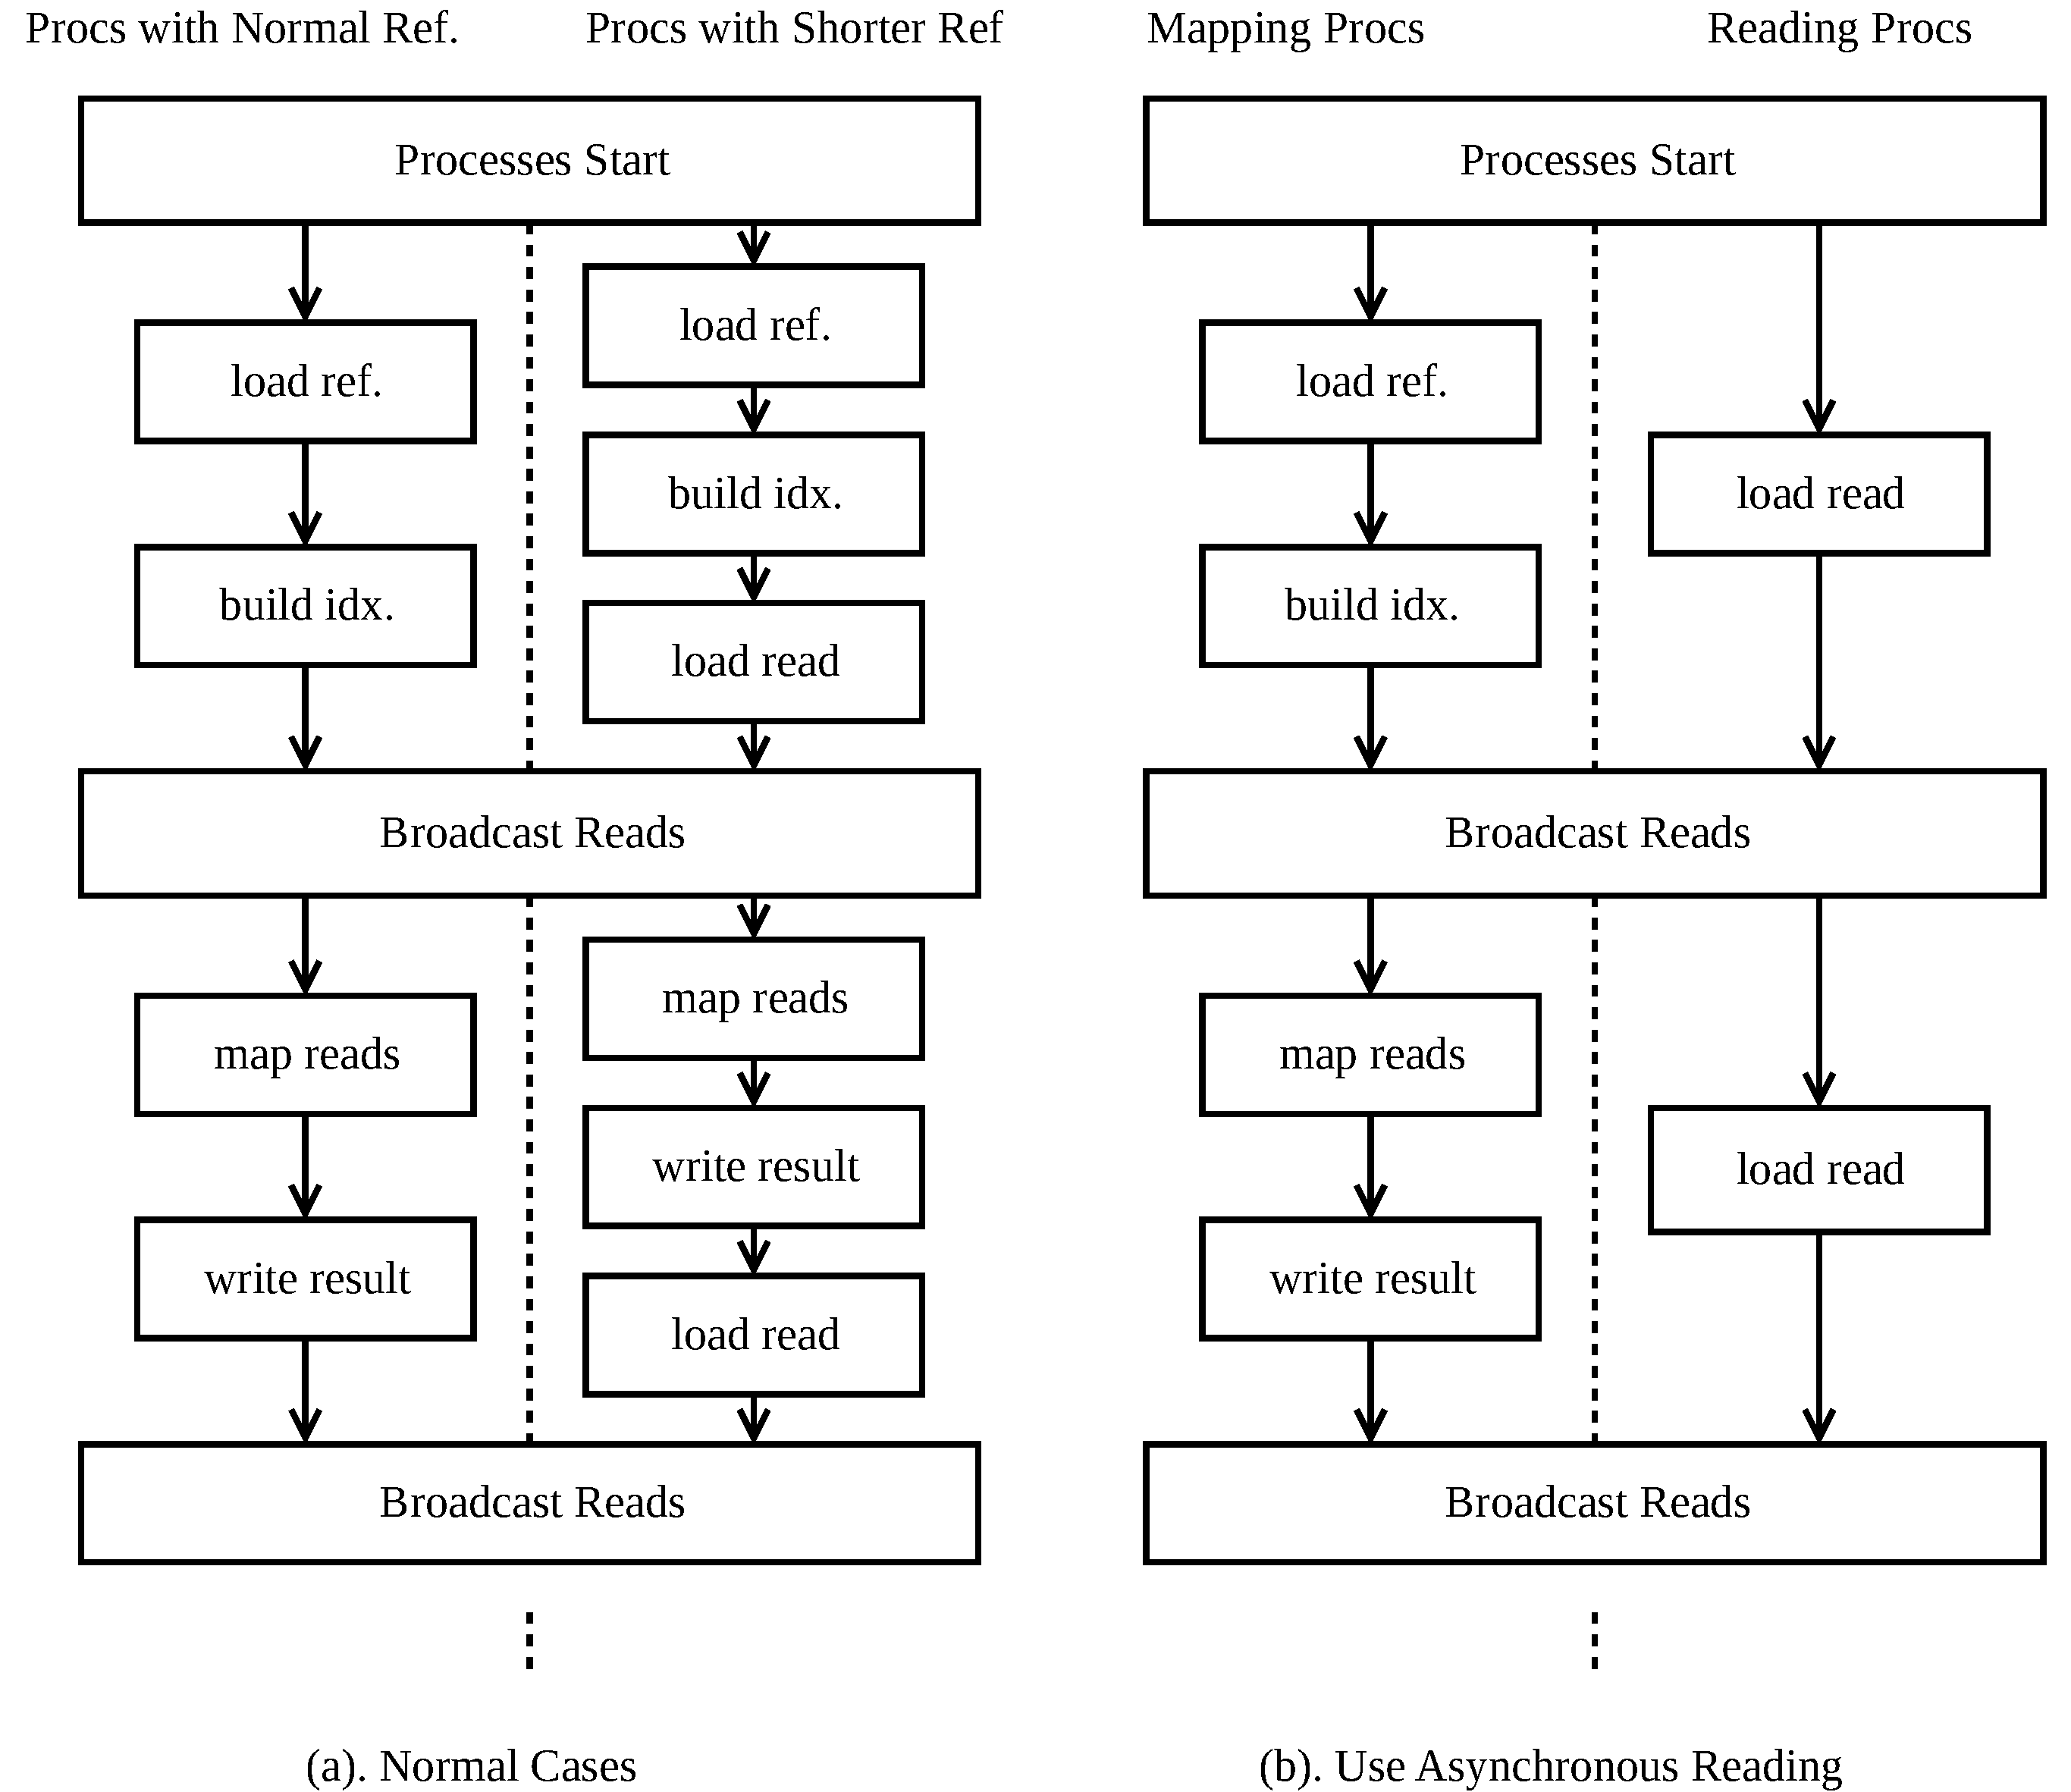
\includegraphics[width=\linewidth]{figures/AsyncRead}
  \caption{Asynchronous data loading strategy: (a) default case, and
    (b) case when there is no significantly shorter reference block.}
  \label{AsyncRead}
\end{figure}

Our reference genome partitioning strategy illustrated in
Figure~\ref{RefDiv} often generates one reference genome block that is
significantly shorter than the others. This block is assigned to the
first row of our task grid. Thus, processes in the first row take less
time during computation and will have sufficient time to load reads
for the subsequent round of computation. This approach therefore
reduces the idle time of other processes waiting for read data.
Figure \ref{AsyncRead}(a) illustrates this strategy.

We further provide an optional asynchronous data-loading strategy in
case that there is no significantly shorter reference block. In this
case we add a row of processes that loads only reads. When other
processes in the column are computing alignments, these processes
exclusively load new read chunks. After loading and computation have
been completed, all processes within a column receive the loaded data
by means of an \texttt{MPI\textunderscore Bcast}. In our experiments,
this approach reduces the idle time between computing two read chunks
by over 90\% when using 8 processes. Figure \ref{AsyncRead}(b)
illustrates this strategy.

\subsection{Multithreaded Intra-CG Parallelization}

\begin{figure}[!htb]
  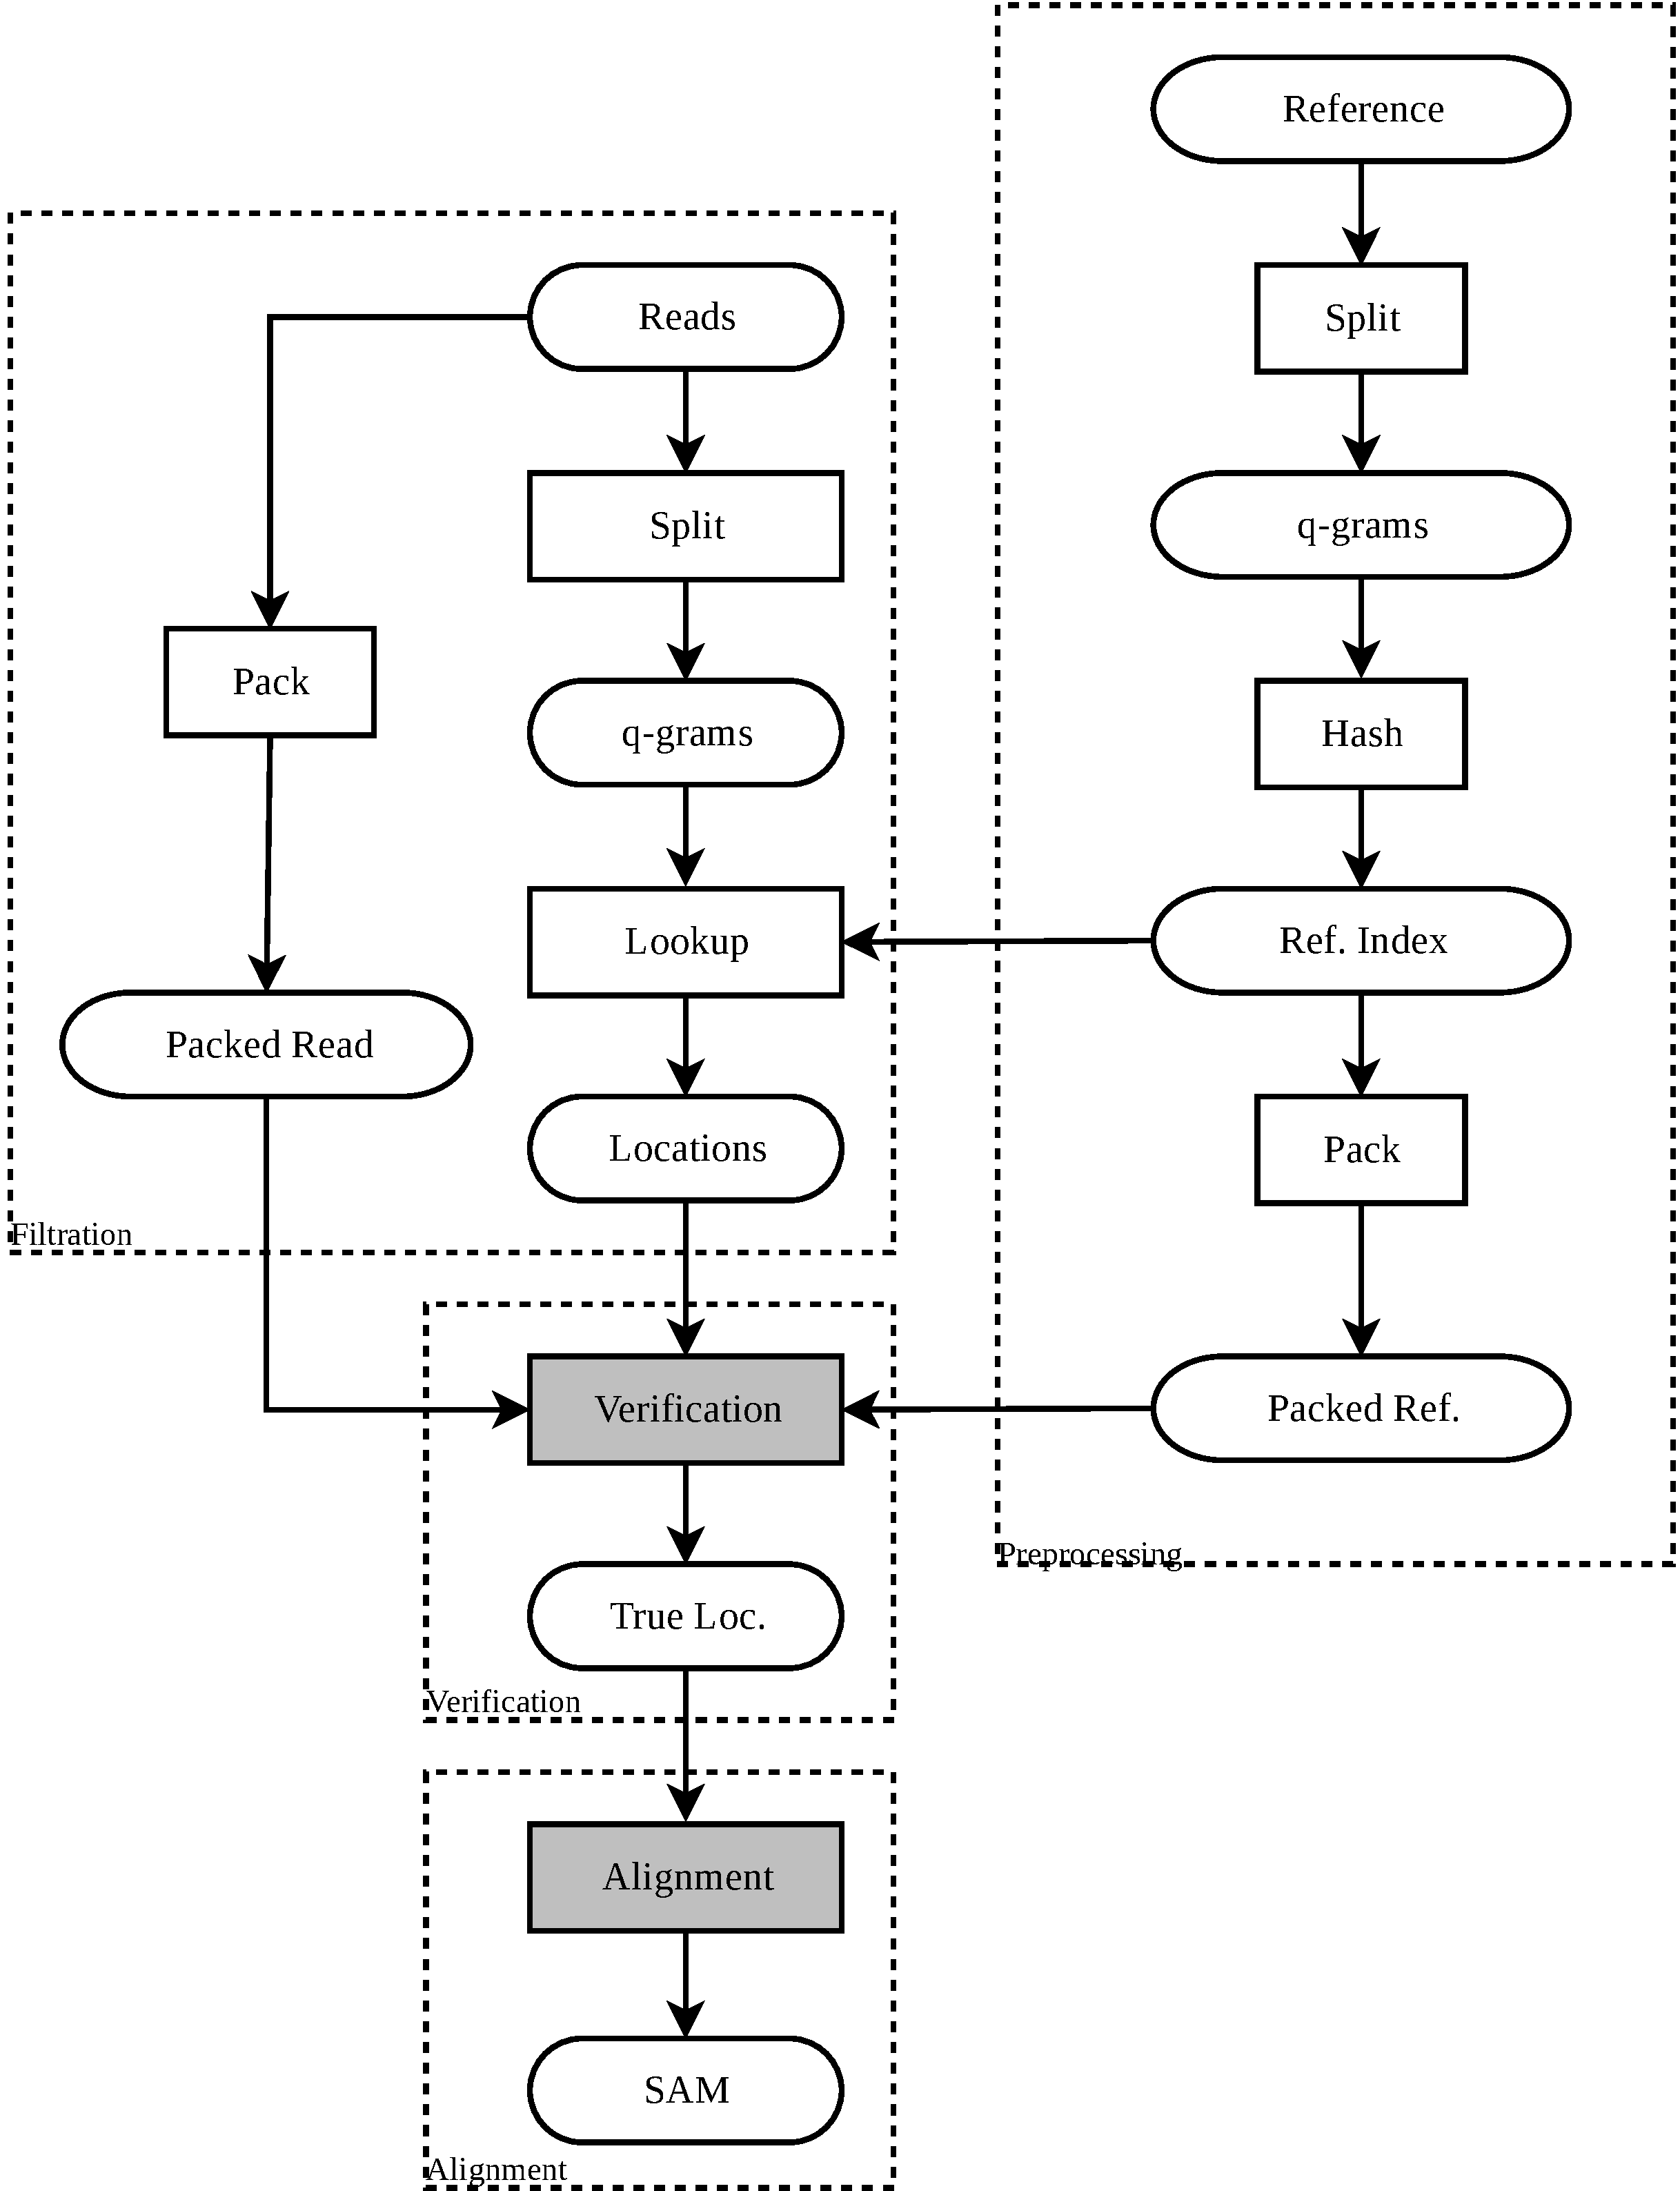
\includegraphics[width=1\linewidth]{figures/FrmWk}
  \caption{Workflow of S-Aligner on a single CG: gray boxes correspond
    to tasks assigned to SPs while tasks in white boxes are executed
    on the MP.}
  \label{FrmWk}
\end{figure}

The second level of parallelism exploits the threading capabilities of
a CG. Our design within a single node is a comprehensive read mapper
based on the described seed-and-extend approach using the three-stage
pipeline: filtration, verification, and alignment. The filtration step
uses a look-up table of $q$-grams of the assigned reference genome
block that can be loaded from a preprocessed index file or
alternatively calculated on-the-fly by a radix sort-based hash table
construction method. After the MP performs the lookup of each
non-overlapping $q$-gram of a read, it stores the retrieved intervals
in a SIMD-friendly manner allowing for efficient vectorization during
the subsequent verification step on the SPs. Verification selects all
intervals that comply with the restricted edit distance using Myers'
bit-parallel algorithm. Afterwards, we employ a banded version of the
Smith-Waterman algorithm on the SPs to align the remaining intervals
that have passed verification. Figure~\ref{FrmWk} shows the workflow
of our intra-CG implementation.

\begin{figure}[!htb]
  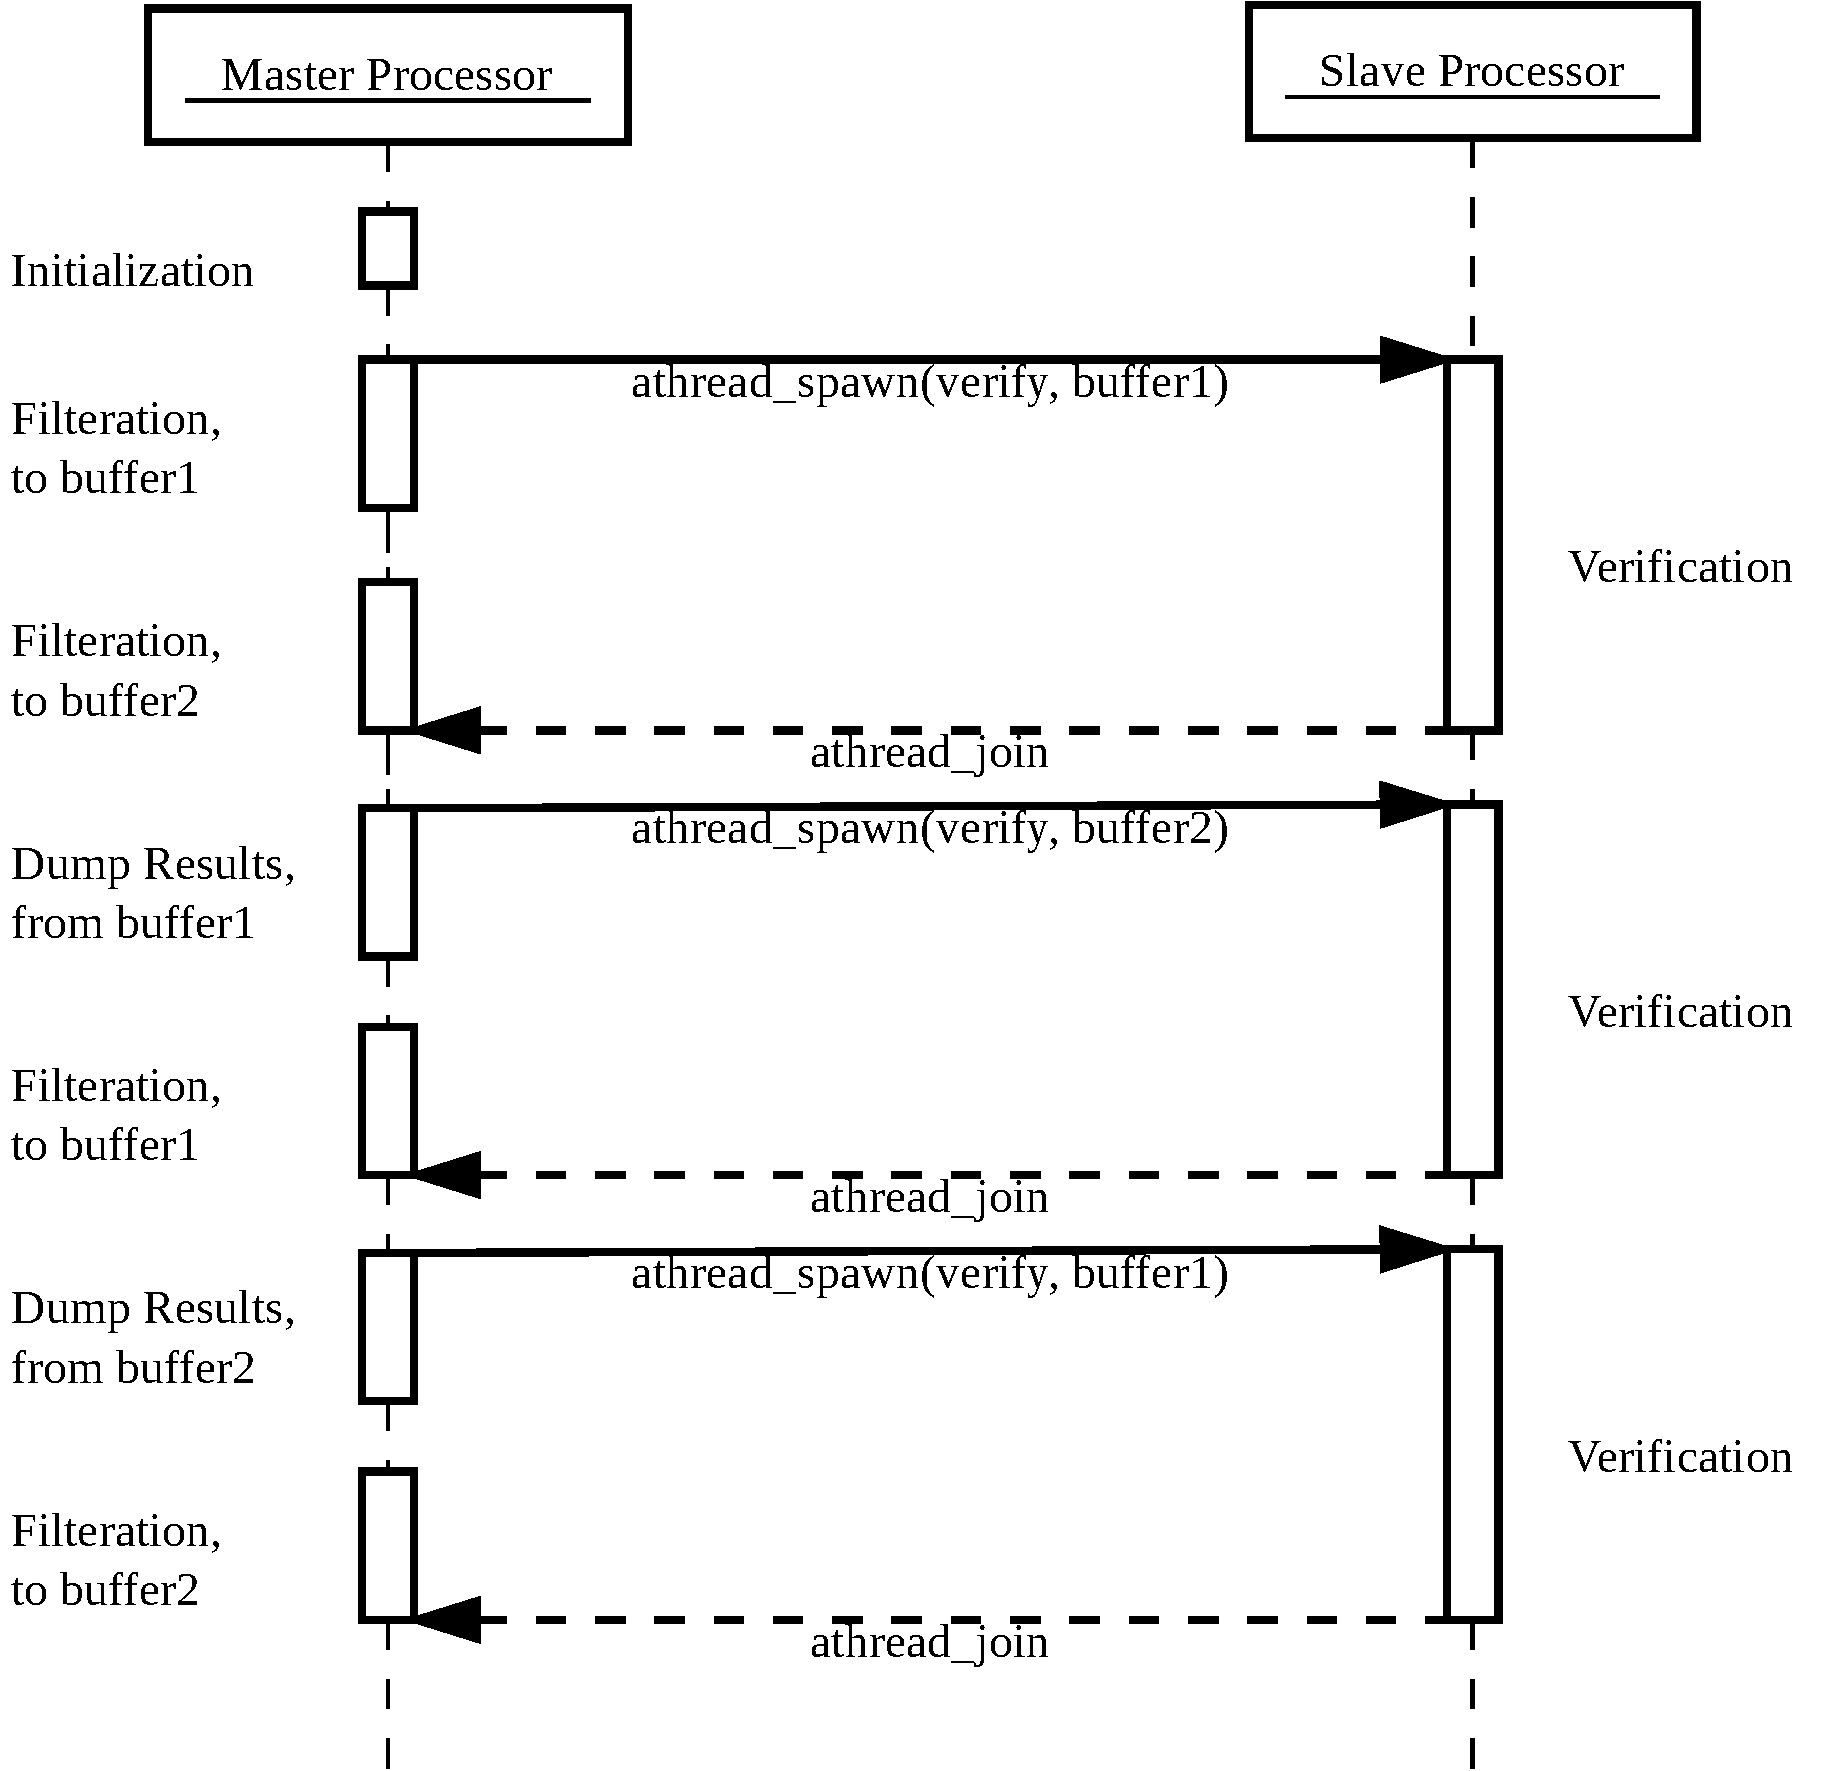
\includegraphics[width=1\linewidth]{figures/AsyncPara}
  \caption{Asynchronous filtration.}
  \label{AsyncPara}
\end{figure}

The intra-CG parallelization is realized by a task parallelization
scheme implemented using spawn and join calls of the {\em athread}
library. The MP executes the filtration stage while the SPs process
the verification step. Each read is divided into non-overlapping
$q$-grams. The MP looks up those $q$-grams in the reference genome
index and returns a number of intervals. The MP copies them to a
buffer that is transferred to the LDM of SPs for verification. We
employ a dual buffer strategy by allocating two buffers for storing
the intervals identified by the MP. When the MP has finished filling
one buffer, it waits for the SP thread group to join, and then
dispatches an SP thread group to verify these intervals. Subsequently,
the MP fills another buffer, while the SP thread group performs
verification. These steps are repeated until all reads are processed
(see Figure \ref{AsyncPara}). The dual buffer strategy reduces the
idle times of SPs and is also used for implementing the subsequent
alignment stage.

\begin{figure}[!htb]
  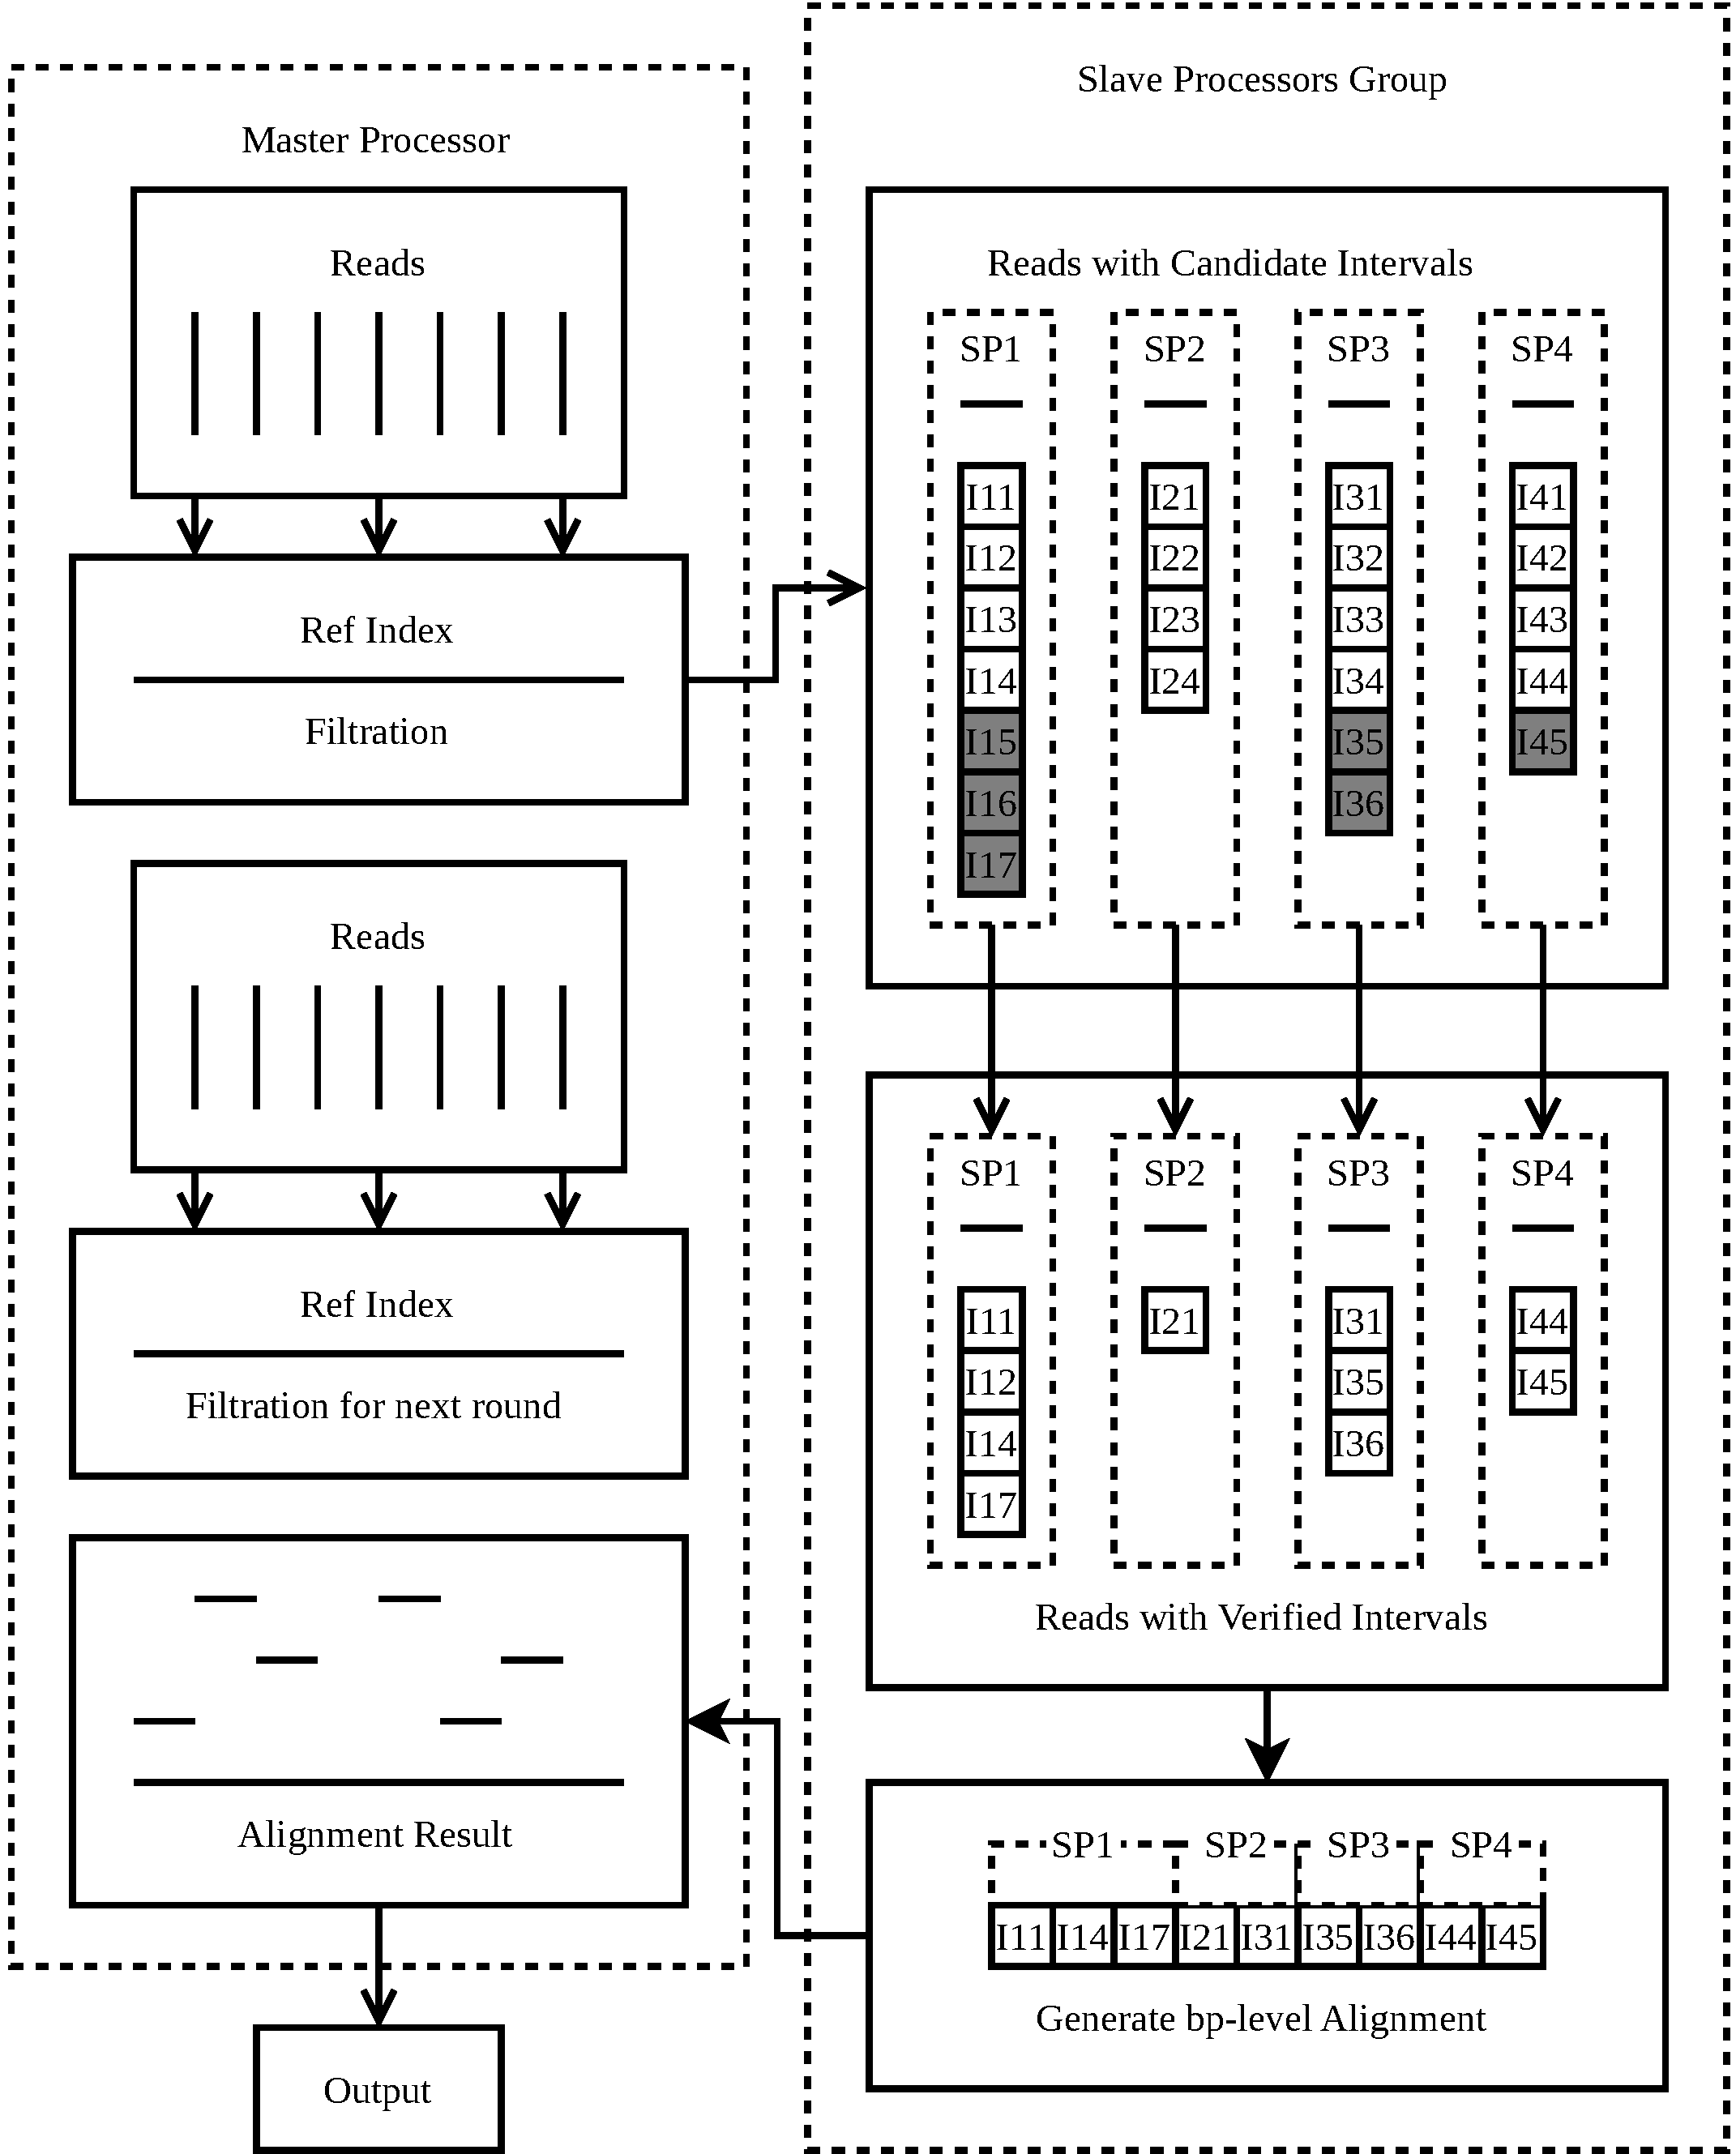
\includegraphics[width=\linewidth]{figures/SPParallel}
  \caption{Framework of our parallelization scheme within one CG: the
    MP performs filtration and output of alignment results while SPs
    verify identified candidate locations and generate base-pair level
    alignments. Gray boxes indicate the intervals verified in the
    second round of verification (assuming $slice\_num = 4$).}
  \label{SPParallel}
\end{figure}

Figure~\ref{SPParallel} illustrates our framework for dividing the
computation between the MP and SPs within a single CG. The number of
seeds identified for a given read can vary while the verification time
of a single seed is constant. Thus, a simple static assignment of seed
intervals per read to SPs can cause workload imbalance.  To balance
the workload, we introduce the parameter $slice\_num$, which restricts
the maximum number of seed intervals to be verified for one read. If
there are more than $slice\_num$ seed intervals to be verified for a
read, we spawn verification threads with the first $slice\_num$
intervals. The remaining intervals will be verified in a subsequent
round of spawns. A value of $slice\_num$ that is too large can reduce
the overhead of spawning SP thread groups, but it worsens workload
balance, and vice versa. Our default value of $slice\_num = 100$
provides a good trade-off in practice.


\subsection{SIMD Vectorization}

Implementing Myers' bit-parallel algorithm using ShenWei's SIMD
intrinsics requires a bit-level encoding of DNA sequences to
efficiently evaluate the characteristic function $\chi(s_{i-1} =
s'_{j-1})$ for all $i, j$.

Different approaches have been used in existing aligners: BWA
\cite{bwa} employs an {\em array of structures} (AoS) while RazerS3
\cite{razers3} stores a DNA sequence in a profile using one-hot
encoding. While the AoS approach is more space-efficient and
cache-friendly, the usage of a profile with one-hot encoding supports
bit-parallel computation in a more efficient way.  Because of the
small size of the LDM and the requirement of bit parallelism, we
employ an encoding strategy that combines an AoS with an SoA ({\em
  structure of arrays}) approach, which we call an AoSoA ({\em array
  of structures of arrays}). This mixed strategy builds two
bit-vectors in an interleaved fashion. Thus, we can fetch the encoded
sequence by one DMA-intrinsic and calculate $\chi(s_{i-1} = s'_{j-1})$
in terms of two logical equality operations. Figure~\ref{MixPack}
illustrates the encoding strategy.

\begin{figure}[!htb]
  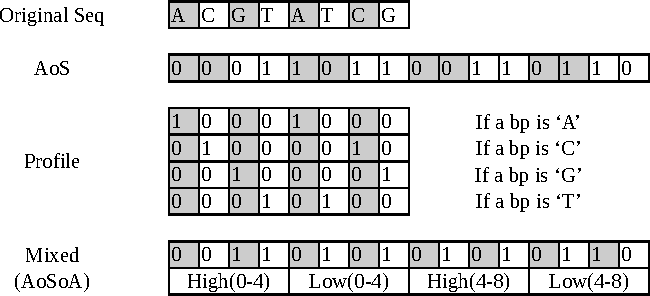
\includegraphics[width=0.9\linewidth]{figures/MixPack}
  \caption{Bit-level encoding strategies for DNA sequences. For
    simplicity, we use a 4-bit word instead of 64-bit word for
    illustrating our combined AoSoA strategy (bottom).}
  \label{MixPack}
\end{figure}

When updating the five bit-vectors according to
Equation~\ref{one-hot-myers} along the columns in a bit-parallel
fashion, a circular dependency needs to be resolved: $D^0_{i,j}$
depends on $H^-_{i-1, j}$, which in turn depends on $D^0_{i-1,j}$ (a
value we have not computed yet). Myers \cite{myers} has shown that
this can be solved by using logical operations and an
addition. ShenWei's SIMD instructions support 256-bit integer
arithmetic, such as \texttt{simd\_uaddo\_take\_carry} (short for SIMD
unsigned octa-word add, taking carry) which adds two 256-bit operands
and returns a 256-bit unsigned integer. Thus, different from
implementations of Myers' algorithm on other architectures (e.g.,
\cite{chacon}), our implementation does not require additional
instructions to process carries generated within a SIMD
lane. Unfortunately, there is no 256-bit compare instruction. Thus, we
have implemented comparisons in terms of shifting operations.

Furthermore, we have simplified the core loop as much as possible in
order to avoid branching statements. This action results in an
implementation consisting of 23 intrinsics as shown in Figure
\ref{cores}, where \texttt{resi32} is set to $|read|\mod 32 - 1$.

\begin{figure}[!htb]
    \begin{lstlisting}[frame=single, xleftmargin=3.5ex]
t1    = simd_vxorw(ref_hi,read_hi[k]);
t2    = simd_vxorw(ref_lo,read_lo[k]);
X     = simd_vbisw(t1,t2); 
X     = simd_vxorw(X,one); 
X     = simd_vbisw(X,VP[k]);
D0    = simd_vandw(X,VP[k]);
D0    = simd_uaddo_take_carry(D0,VP[k]);
D0    = simd_vandw(D0,VP[k]);
D0    = simd_vandw(D0,X);
HN    = simd_vandw(VP[k],D0);
HP    = simd_vbisw(VP[k],D0);
HP    = simd_vxorw(HP,one);
HP    = simd_vbisw(HP,VN[k]);	
X     = simd_sllow(HP,resi32);
X     = simd_vbisw(X,pr_HP);
pr_HP = simd_srlow(HP,255);
VN[k] = simd_vandw(X,D0);
VP[k] = simd_vbisw(X,D0);
VP[k] = simd_vxorw(VP[k],one);
t2    = simd_sllow(HN,resi32);
t2    = simd_vbisw(t2,pr_HN);
pr_HN = simd_srlow(HN,255);
VP[k] = simd_vbisw(t2,VP[k]);	
    \end{lstlisting}
    \caption{SIMD core instructions used to implement Myers' algorithm
      on ShenWei. The reference sequence is presented as
      \texttt{ref\_hi}, the high-bit of the pattern, and
      \texttt{ref\_lo}, the low-bit of the pattern. The read sequence
      is stored in the vectors \texttt{read\_hi[k]} and
      \texttt{read\_lo[k]}. The variables \texttt{D0}, \texttt{HN},
      \texttt{HP}, \texttt{VN}, \texttt{VP} refer to the corresponding
      variables in Equation~\ref{one-hot-myers}.}
    \label{cores}
\end{figure}

\subsection{Exploiting Local Device Memory}

\begin{figure}[!htb]
  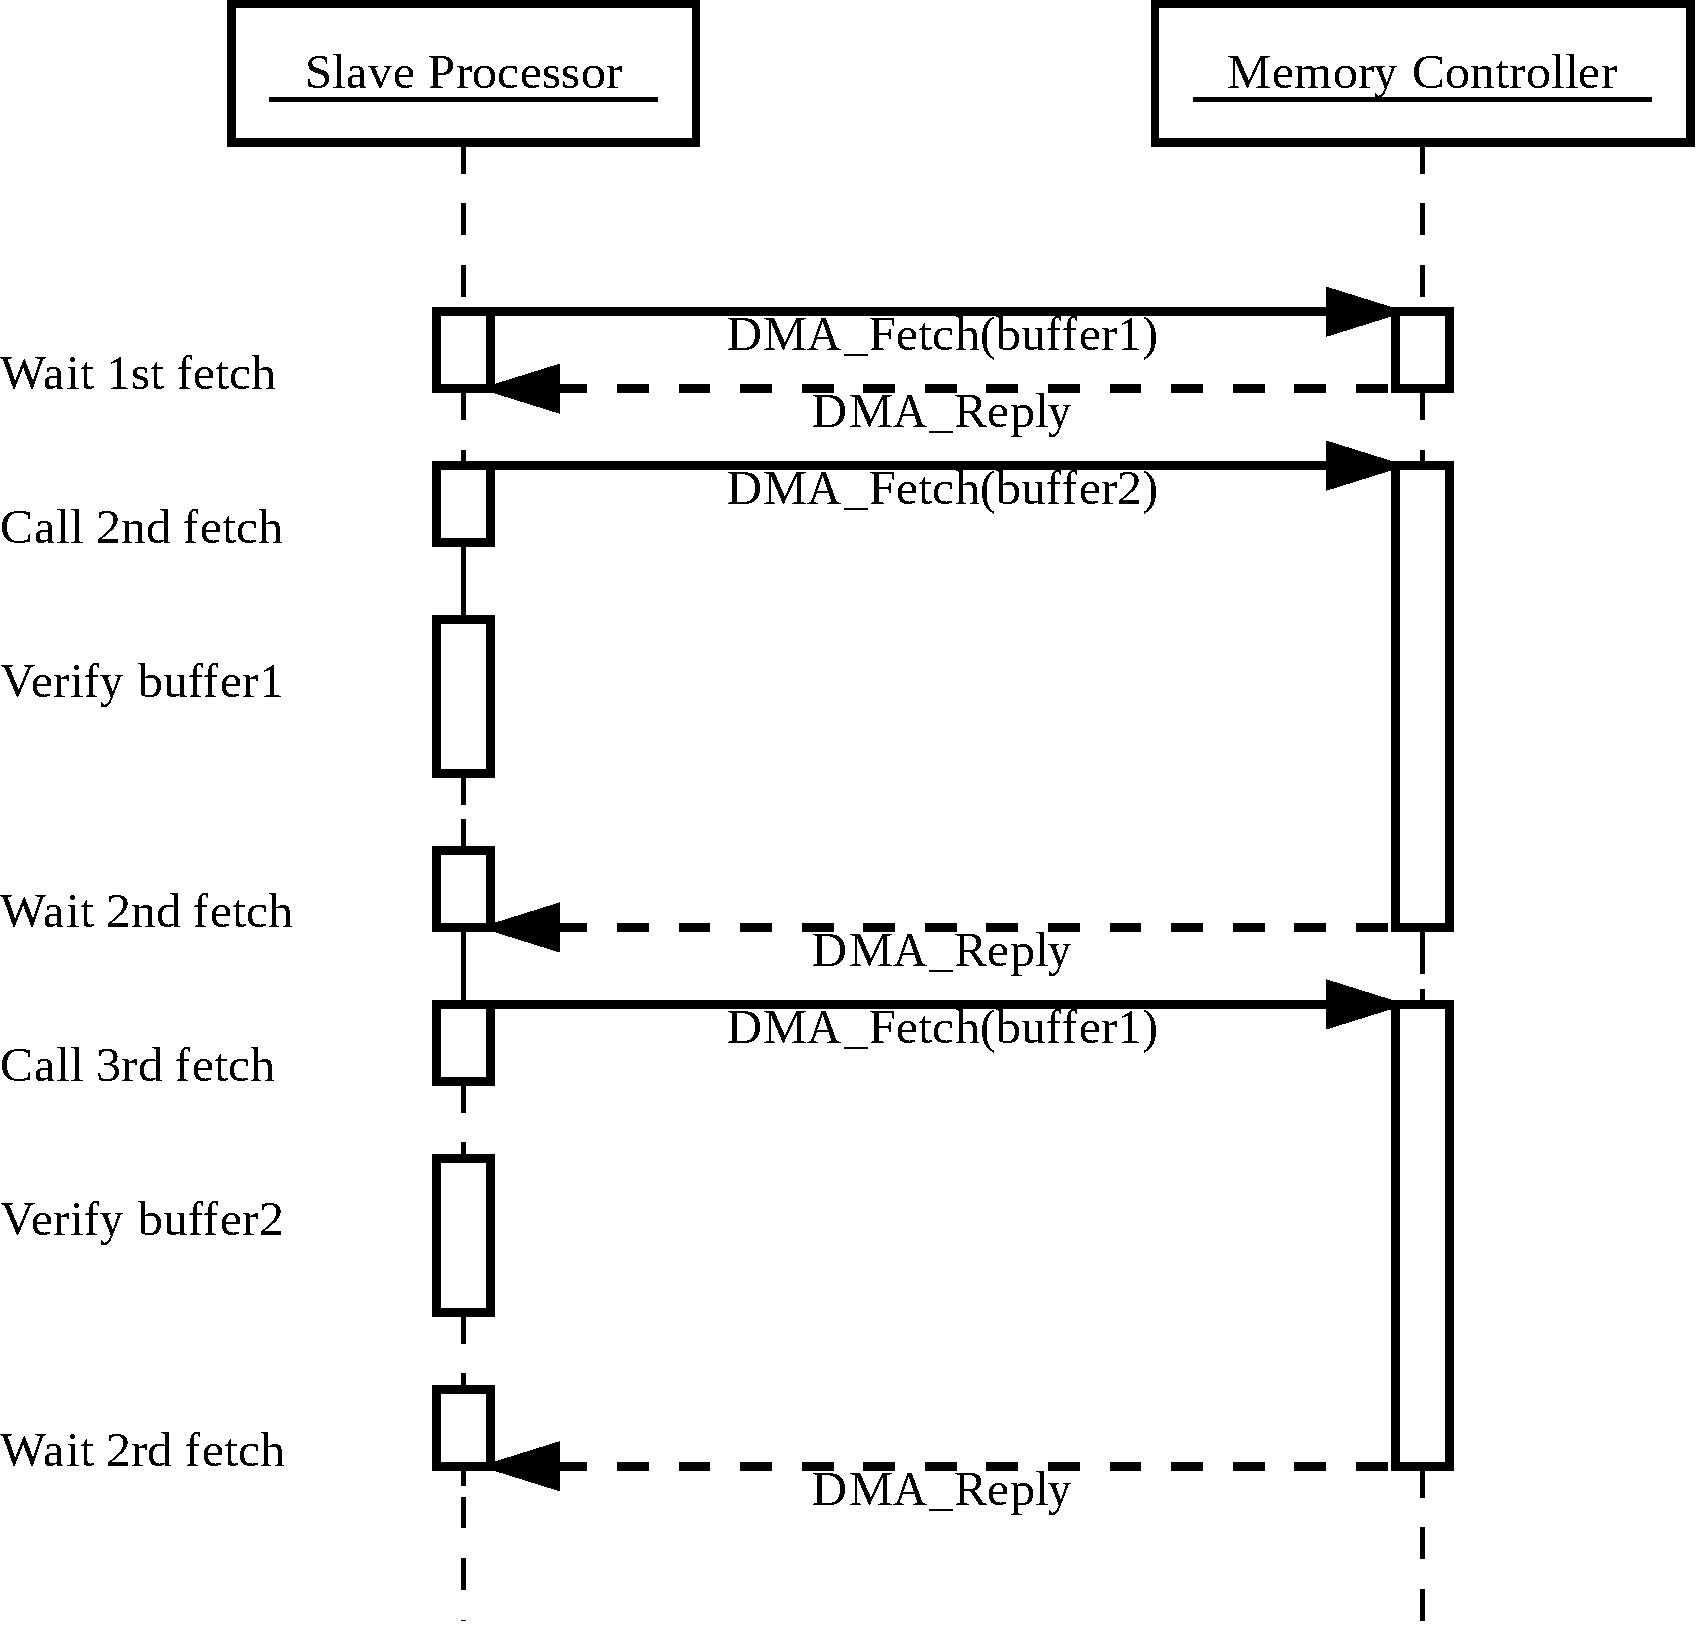
\includegraphics[width=1\linewidth]{figures/AsyncTrans}
  \caption{Asynchronous data transfer to LDM.}
  \label{AsyncTrans}
\end{figure}

Since SPs do not have any cache and the latency to access the DDR3
shared memory is high, the usage of the explicitly managed LDM is
crucial.  DMA fetching is the most efficient way to transfer data
between main memory and LDM (i.e., significantly faster than using
functions such as \texttt{memcpy}). DMA calls are handled by the
memory controller, and SPs can continue to perform computation. Thus,
we can overlap data transfers from shared memory to LDM and the
verification of intervals using Myers' algorithm by using asynchronous
DMA-fetching intrinsics presented by ShenWei.

Figure \ref{AsyncTrans} shows our framework for asynchronous data
transfer from DDR3 shared main memory to the LDM of SPs. We allocate
two buffers in LDM. When an interval in one buffer is verified, the
subsequent interval is being fetched to the other buffer using DMA
intrinsics. The SP busy-waits for the completion of DMA-fetching
before it starts the next verification.

Here we use a busy-waiting strategy because the time used for DMA
fetching is usually shorter than the time required for
verification. Thus, in the common case the DMA reply word needs to be
checked just once in order to pass the busy-wait loop. Our
experimental results show that our asynchronous data transfer
implementation can almost hide the DMA-fetching latency completely and
gains a performance improvement of a factor of 22 compared with an
implementation based on \texttt{memcpy}.

\section{Performance Evaluation}
\label{Evaluation}

The performance of S-Aligner has been evaluated on the Sunway Taihu
Light supercomputer. We use GRCh38\footnote{available at
  http://hgdownload.cse.ucsc.\\edu/downloads.html} as the human
reference genome.  For the read input data sets we use either
ERR013135\footnote{available at
  ftp://ftp.sra.ebi.ac.uk/vol1/fastq/ERR013/\\ERR013135} or reads
simulated by Mason \cite{mason} or wgsim \cite{wgsim}.\footnote{Note
  that Mason usually generates reads of higher quality but does not
  support long reads.}  We first evaluate the performance in terms of
runtime and mapping accuracy on a single node. Subsequently, we
evaluate the scalability of our implementation by varying the number
of utilized nodes up to 13,312.

\subsection{Single-Node Performance Analysis}

In our single-node experiment, we used the first chromosome of GRCh38 as
reference and 20K reads of length 200 bps generated by Mason as input
data.

First, we evaluated the runtime performance of four different
implementations of edit distance calculation using Myers' algorithm in
one CG: (1) a na\"ive method using the MP only, (2) a na\"ive method
with a nonvectorized SP parallelization, (3) a vectorized Myers
algorithm with the MP only, and (4) our vectorized Myers algorithm
with SP parallelization.

\begin{figure}[!htb]
  \begin{center}
    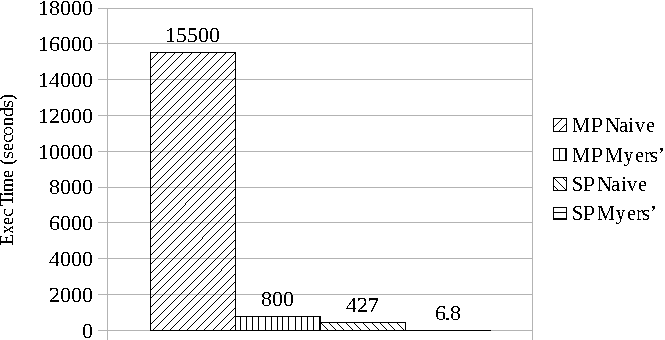
\includegraphics[width=1\linewidth]{figures/VarVerCha}
    \caption{Comparison of the runtimes of four implementations of
      Myers' algorithm on a single CG.}
    \label{VarVerCha}
  \end{center}
\end{figure}

The results in Figure \ref{VarVerCha} show that making
full use of SPs and bit-parallel SIMD vectorization gains dramatic
speedups (118$\times$ and 63$\times$, respectively). Since the MP does
not support high-precision (256-bit integer) extensions, we
implemented a workaround for the high-precision addition
operation. This makes it run slower on a single MP than on a single
SP. Thus, using SPs can gain a superlinear speedup in this
application. Furthermore, our bit-parallel SIMD implementation is able
to update 256 cells simultaneously using 23 instructions (i.e., 0.09
instructions per cell) while the na\"ive implementation computes one
cell using 6 instructions. This results in a theoretical speedup of
$\sim$67$\times$, which explains the actually achieved speedup of
63$\times$.

Second, we evaluated the impact of using asynchronous filtration and
the impact of using DMA intrinsics versus \texttt{memcpy}. The results
are shown in Figure \ref{VarOptCha}.

\begin{figure}[!htb]
  \begin{center}
    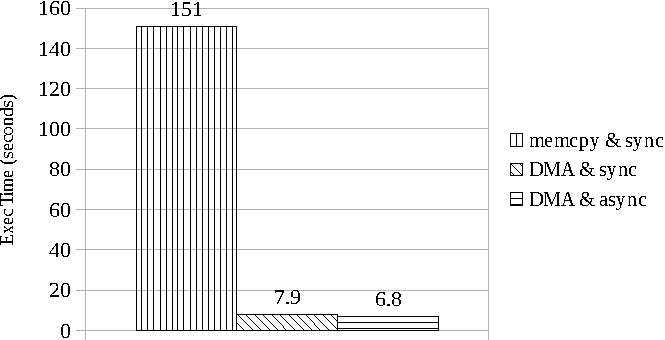
\includegraphics[width=1\linewidth]{figures/VarOptCha}
    \caption{Evaluation with and without I/O optimizations.}
    \label{VarOptCha}
  \end{center}
\end{figure}

The results demonstrate that DMA fetching is key for achieving high
performance when using SPs, since a speedup of $\sim$22$\times$ is
gained over \texttt{memcpy}. This can be attributed to two factors:
(1) DMA transfers require fewer compute resources since they are
performed by the memory controller, whereas \texttt{memcpy} uses an SP
to write data to memory; and (2) DMA fetching can be performed
asynchronously, thus enabling the latency of fetching data to be
hidden by computation. Furthermore, asynchronous filtration gains
$\sim$15\% speedup.

In summary, the architecture of SW26010 differs significantly from a
conventional x86\_64 CPU. Straightforward migration of code therefore
typically results in an inefficient implementation on SW26010, and
architecture-specific optimizations are required in order to achieve
high performance. As a case study, we compiled and executed
multithreaded BWA \cite{bwa} (one of the most well-known {\em any-best
  mappers}) on SW26010. It runs two times slower than S-Aligner, while
finding significantly fewer locations, showing the importance of
making changes according to this specific architecture.

\subsection{Comparison with RazerS3}

In our experiment with RazerS3, we used the first chromosome from GRCh38 as
reference and various numbers of reads from ERR013135. The runtime of
S-Aligner on a single SW26010 node was compared with that of RazerS3, a
representative all-mapper. Since RazerS3 does not support ShenWei's
architecture, we ran it on a machine with Intel processors using
multithreading with default parameters (e.g., the accuracy parameter
is set to 98\%). Measured runtimes are shown in Table
\ref{SingleNode}.  One can see that S-Aligner executed on a single
SW26010 (260 cores running at 1.45 GHz) outperforms RazerS3 running on
eight Xeon E7-8860v3 CPUs (128 cores running at 3.2 GHz).

\begin{table}
  \begin{threeparttable}
    \caption{Runtime comparison between S-Aligner running on a single
      node with 4 CGs and RazerS3 running on a single node with eight Xeon
      E7-8860v3 CPUs.}
    \label{SingleNode}
    \begin{tabular}{@{\extracolsep{2pt}}rrrrr}
      \hline
      \multicolumn{1}{c}{Ref} &
      \multicolumn{2}{c}{Reads} &
      \multicolumn{2}{c}{Time(s)}\\
      \cline{2-3}
      \cline{4-5}
      \multicolumn{1}{c}{\#bps} &
      \multicolumn{1}{c}{Count} &
      \multicolumn{1}{c}{\#bps} &
      \multicolumn{1}{c}{RazerS3\tnote{\textdagger}} &
      \multicolumn{1}{c}{S-Aligner\tnote{\textdaggerdbl}}\\
      \hline
      116M & 40M & 108 &  939 & 405\\
      253M & 40M & 108 &  3,044 & 892\\
      253M & 40M & 200 &  3,430 & 2,580\\
      \hline
    \end{tabular}
    \begin{tablenotes}
    \item[\textdagger] Result is from a machine with eight Xeon
      E7-8860v3 (128 cores up to 3.20 GHz).
    \item[\textdaggerdbl] Result is from a node with a SW26010 (260
      cores with frequency of 1.45 GHz).
    \end{tablenotes}
  \end{threeparttable}
\end{table}

Rabema \cite{rabema} (Read Alignment BEnchMark) is a well-defined read
alignment benchmark that can evaluate the quality of read mappers in
both {\em all} and {\em any-best} mode. We evaluated the accuracy of
S-Aligner in {\em all} mode based on Rabema by using the result of RazerS3
with the accuracy parameter set to 100\% as gold standard. S-Aligner
can find up to 99.8\% of the normalized intervals found by RazerS3
(100\% accuracy), which is higher than the accuracy of RazerS3
executed with default parameters (98\% accuracy). Detailed results are
provided in Table~\ref{AccuEval}.

\begin{table}
  \begin{threeparttable}
    \caption{Accuracy evaluation of S-Aligner for both real and
      simulated data.}
    \label{AccuEval}
    \begin{tabular}{@{\extracolsep{2pt}}rrrrrr}
      \hline
      \multicolumn{1}{c}{Chrom} &
      \multicolumn{3}{c}{Reads} &
      \multicolumn{1}{c}{\multirow{2}{*}{Interv. found}} \\
      \cline{2-4}
      \multicolumn{1}{c}{Index} &
      \multicolumn{1}{c}{Origin} &
      \multicolumn{1}{c}{Count} &
      \multicolumn{1}{c}{\#bps} \\		
      \hline
      1\textsuperscript{st} & ERR013135 & 20,000 & 108 & 99.34\%\\
      1\textsuperscript{st} & Mason &  20,000 & 200 & 99.82\%\\
      \hline
    \end{tabular}
  \end{threeparttable}
\end{table}

\subsection{Scalability Analysis}

To evaluate weak and strong scalability, we measured the runtimes of
S-Aligner using different numbers of nodes ranging from 13 to
13,312. The full GRCh38 assembly of the human genome was used as
reference. Input reads were simulated by Mason with an error rate of
4\% and a length of 200 bps. Weak scalability was measured for numbers
of nodes ranging from 13 to 3,328 by increasing the number of input
reads from 16 million to 4 billion, correspondingly. Strong
scalability was measured by increasing the number of nodes from 3,328
to 13,312 while keeping the number of input reads constant at 4
billion. We measured the performance in terms of {\em read base-pairs
  processed per second} in total and normalized per node (see
Table \ref{paraexp}). Figure \ref{VarProcCha} shows the achieved
speedups and efficiencies. The results demonstrate weak scalability
since the normalized node performance is almost constant for the
number of nodes ranging from 13 to 3,328. Furthermore, the node
performance only slightly decreases when increasing the number of
nodes from 3,328 to 13,312 while keeping the number of input reads
constant at 4 billion, thus demonstrating strong scalability for
sufficiently large input datasets.

\begin{table}[!htb]
  \begin{threeparttable}
    \caption{Performance and runtime evaluation of S-Aligner using
      different numbers of nodes.}
    \label{paraexp}
    \begin{tabular}{rrrrrr}
      \hline
      \multicolumn{1}{c}{\multirow{2}{*}{\# Nodes}} &
      \multicolumn{2}{c}{Reads}  &
      \multicolumn{1}{c}{\multirow{2}{*}{Time(s)}} &
      \multicolumn{2}{c}{Performance (bpps)} \\
      \cline{2-3}
      \cline{5-6}
      \multicolumn{1}{c}{} &
      \multicolumn{1}{c}{Count} &
      \multicolumn{1}{c}{\# bps} & &
      \multicolumn{1}{c}{Total (M)} &
      \multicolumn{1}{c}{Node (K)}\\
      \hline
      13 & 16M & 200 & 1,315 & 2.43 & 185.43\\
      52 & 64M & 200 & 1,321 & 9.69 & 184.80\\
      208 & 256M & 200 & 1,321 & 38.76 & 184.66\\
      832 & 1,024M & 200 & 1,327 & 154.33 & 184.59\\
      3,328 & 4,096M & 200 & 1,349 & 607.26 & 179.67\\
      13,312 & 4,096M & 200 & 344 & 2,381.40 & 178.90\\
      \hline
    \end{tabular}
    \begin{tablenotes}
    \item
      \# Nodes is the number of nodes involved in computing..
    \item
      bpps is short for million base pairs processed per second.
    \item
      M (K) indicates that column is presented in millions (thousands).
    \end{tablenotes}
  \end{threeparttable}
\end{table}

\begin{figure}[!htb]
  \begin{center}
    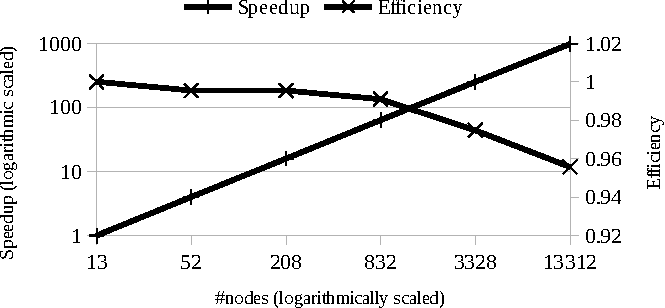
\includegraphics[width=1\linewidth]{figures/VarProcCha}
    \caption{Speedup and efficiency of S-Aligner for different numbers
      of nodes.}
    \label{VarProcCha}
  \end{center}
\end{figure}

\section{Conclusion}
\label{Conclusion}

NGS data will continue to grow rapidly in the foreseeable future. Read
mapping is a critical and compute-intensive step for a variety of NGS
pipelines. While significant efforts have been devoted to optimizing
this task, it is still a major bottleneck. In this paper, we have
introduced S-Aligner---a highly scalable read mapper specifically
designed to fit the characteristics of the Sunway Taihu Light
supercomputer and its SW26010 architecture.  It scales almost linearly
with over 95\% parallelization efficiency when distributed over more
than 50,000 processes. As a result, S-Aligner can map $\approx$ 1.6 TB
of read data to the whole human genome in just a few
minutes. Moreover, when executed on a single node it can outperform
the popular all-mapper RazerS3 executed on eight Xeon E7-8860 CPUs
while achieving highly competitive mapping accuracy.

From S-Aligner we learn a number of lessons about properly
designing parallelization and communication patterns in order to
achieve both high performance and scalability on the new Sunway Taihu
Light supercomputer. First, both multithreading and SIMD vectorization
must be employed in order to fully exploit the computational resources of
the SW26010 processor. Second, within an SP the fast LDM must be used
via DMA intrinsics in order to guarantee efficient intra-CG
communication. Third, a scalable inter-CG communication scheme must be
implemented in a way that efficiently hides the interconnection
network bottleneck. Fourth, asynchronous file-loading and data-sharing
strategies need to be implemented in order to effectively hide the
latency of the network file system. The techniques presented in this
paper can also be adapted to map similar applications exhibiting a
pipeline of hashing and verification, such as large-scale approximate
near duplicate object detection \cite{efficient} or de novo genome
assembly \cite{swap} onto the heterogeneous many-core cluster
architecture of Sunway Taihu Light.


\section*{Acknowledgment}
This material is based upon work supported by the PPP project from CSC and DAAD, 
Taishan Scholar, and the U.S. Department of Energy, Office of Science, under contract 
DE-AC02-06CH11357.

\bibliographystyle{plain}
\bibliography{bib/references.bib}

\vspace{20pt} \footnotesize{The submitted manuscript has been created
  by UChicago Argonne, LLC, Operator of Argonne National Laboratory
  (``Argonne'').  Argonne, a U.S. Department of Energy Office of
  Science laboratory, is operated under Contract
  No. DE-AC02-06CH11357. The U.S. Government retains for itself, and
  others acting on its behalf, a paid-up nonexclusive, irrevocable
  worldwide license in said article to reproduce, prepare derivative
  works, distribute copies to the public, and perform publicly and
  display publicly, by or on behalf of the Government.  The Department
  of Energy will provide public access to these results of federally
  sponsored research in accordance with the DOE Public Access
  Plan. http://energy.gov/downloads/doe-public-access-plan.}

\end{document}
